%%%% ijcai19.tex

\typeout{IJCAI-19 Instructions for Authors}

% These are the instructions for authors for IJCAI-19.

\documentclass{article}
\pdfpagewidth=8.5in
\pdfpageheight=11in
% The file ijcai19.sty is NOT the same than previous years'
\usepackage{ijcai19}
\usepackage{multirow}
% Use the postscript times font!
\usepackage{times}
\usepackage{soul}
\usepackage{url}
%\usepackage[hidelinks]{hyperref}
\usepackage[utf8]{inputenc}
\usepackage{amssymb, color}
\usepackage[small]{caption}
\usepackage{graphicx, subfig}
\usepackage{amsmath}
\usepackage{booktabs}
\usepackage{algorithm}
\usepackage{algorithmic}
\usepackage{makecell}
\urlstyle{same}
\newcommand{\kai}[1]{\textcolor{blue}{Kai: {#1}}}
\newcommand{\m}{EFN}
\newcommand{\tabincell}[2]{\begin{tabular}{@{}#1@{}}#2\end{tabular}}
\linespread{0.945}
\title{Exploiting Emotions for Fake News Detection on Social Media}
% Single author syntax
%\author{Anonymous
%}
\author{
	Chuan Guo$^{1,3}$\and
	Juan Cao$^{1,3}$\footnote{Contact Author}\and
	Xueyao Zhang$^{1,3}$\and
	Kai Shu$^4$\And
	Miao Yu$^{2}$\\
	\affiliations
	$^1$Key Laboratory of Intelligent Information Processing Center for Advanced Computing Research, Institute of Computing Technology, Chinese Academy of Sciences\\
	$^2$Institute of Information Engineering, Chinese Academy of Sciences\\
	$^3$University of Chinese Academy of Sciences\\
	$^4$Department of Computer Science and Engineering, Arizona State University\\
	\emails
	\{guochuan, caojuan\}@ict.ac.cn,
	xueyao\_98@foxmail.com,
	kai.shu@asu.com,
	yumaio@iie.ac.cn
}
\begin{document}
	
	\maketitle
	
	\begin{abstract}
		%   As microblog become one of the most popular platform where people generate, share and seek information, it also facilitates the generation and propagation of rumors, which could lead serious consequences. 
		Microblog has become a popular platform for people to post, share, and seek information due to its convenience and low cost. However, it also facilitates the generation and propagation of fake news, which could cause detrimental societal consequences. Detecting fake news on microblogs is important for societal good. Emotion is a significant indicator while verifying information on social media. 
		%   In the rumor event, to impress the audience and spread extensively, the publishers typically either post a tweet with intense emotion which could easily resonate with the crowd, or post a controversial statement unemotionally but aim to invoke intense emotion in the crowd, such as anger, shock, and sadness. Thus, emotion can be a important signal that has the potential to detect false rumors on microblogs.
		%   However, existing works using emotion information for false rumor detection are mainly focuses on stance mining or statistical emotional features, which . 
		Existing fake news detection studies utilize emotion mainly through users stances or simple statistical emotional features; and exploiting the emotion information from both news content and user comments is also limited. In the realistic scenarios, to impress the audience and spread extensively, the \textit{publishers} typically either post a tweet with intense emotion which could easily resonate with the crowd, or post a controversial statement unemotionally but aim to evoke intense emotion among the \textit{users}. 
		%  Therefore, in this paper, we deeply explore the importance of emotion and incorporate emotion in the traditional rumor detection apporachs. We define two kinds of emotion, content emotion and social emotion, to capture the emotion of the publishers and the crowds respectively. The proposed approach leverages a weekly labeled emotion weibo corpus for learning emotion representation of each word. And gate mechanism is applied for fusion at both word and mode level. Experiment conducted on real-world weibo datasets demonstrate that our apporach outperforms state-of-art rumor detection approaches.
		Therefore, in this paper, we study the novel problem of exploiting emotion information for fake news detection. We propose a new \underline{E}motion-based \underline{F}ake \underline{N}ews \underline{D}etection framework ({\m}), which can i) learn content- and comment- emotion representations for publishers and users respectively; and ii) exploit content and social emotions simultaneously for fake news detection. Experimental results on real-world dataset demonstrate the effectiveness of the proposed framework.
	\end{abstract}
	
	\section{Introduction}
	
	Social media platforms play a crucial role for people to seek out and spread information, especially in emergencies and breaking news. However, the convenience of publishing and spreading information also foster the wide propagation of \textit{fake news}, commonly referred as intentional false information~\cite{shu2017fake}. %These fake news often occur in various important social issues, such as political events, natural disasters and economic crisis, which seriously misled the audience and raise chaos in public. 
	For instance,  an authoritative analysis of BuzzFeed News\footnote{https://www.buzzfeednews.com/article/craigsilverman/viral-fake-election-news-outperformed-real-news-on-facebook} indicated that, during the 2016 U.S. presidential election campaign, top 20 fake news stories generated more total engagement on Facebook than top 20 major real news, that these fake news earned nearly 9 million shares on social media. These fakes news seriously do harm to not only the public credibility, but also social stability and economic market. Therefore, it's significantly important to build tools to detect the fake news automatically and effectively. 
	%	\kai{fake newss and fake news are different conceptually, you can either use fake news or fake news}
	
	\begin{figure}
		\centering
		\begin{minipage}[t]{0.22\textwidth}
			\subfloat[]{\label{Fig:introcase1}%%
				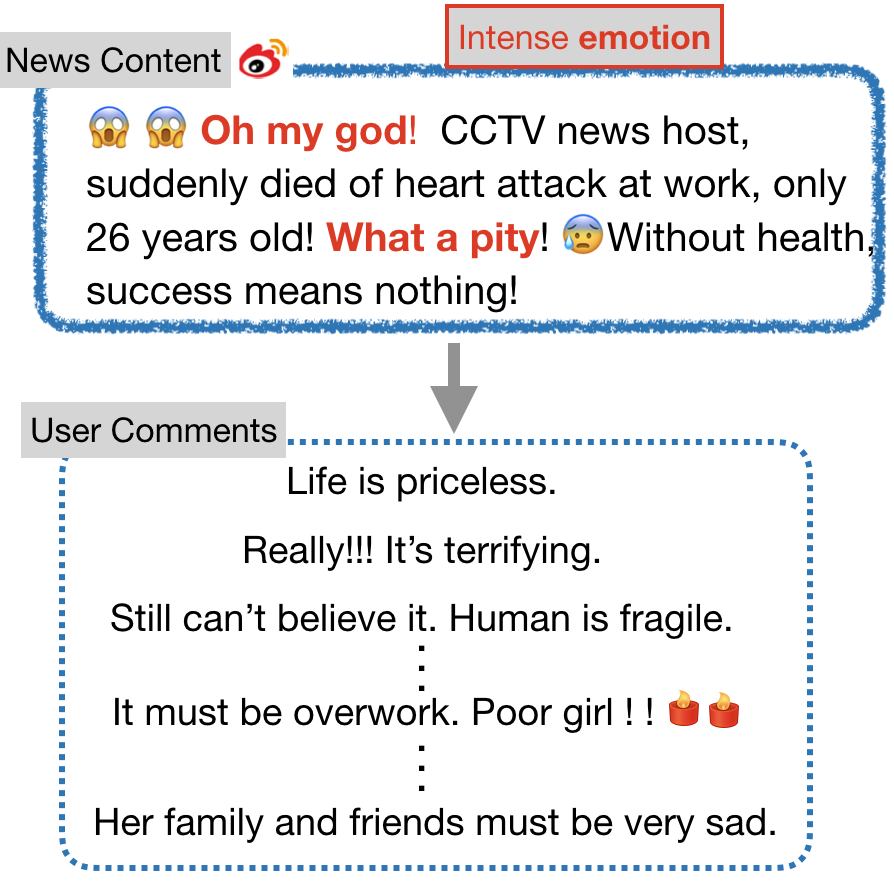
\includegraphics[width=1.6in]{./Figure/introcase1.png}}
		\end{minipage}
		\begin{minipage}[t]{0.23\textwidth}
			\subfloat[]{\label{Fig:introcase2}%%
				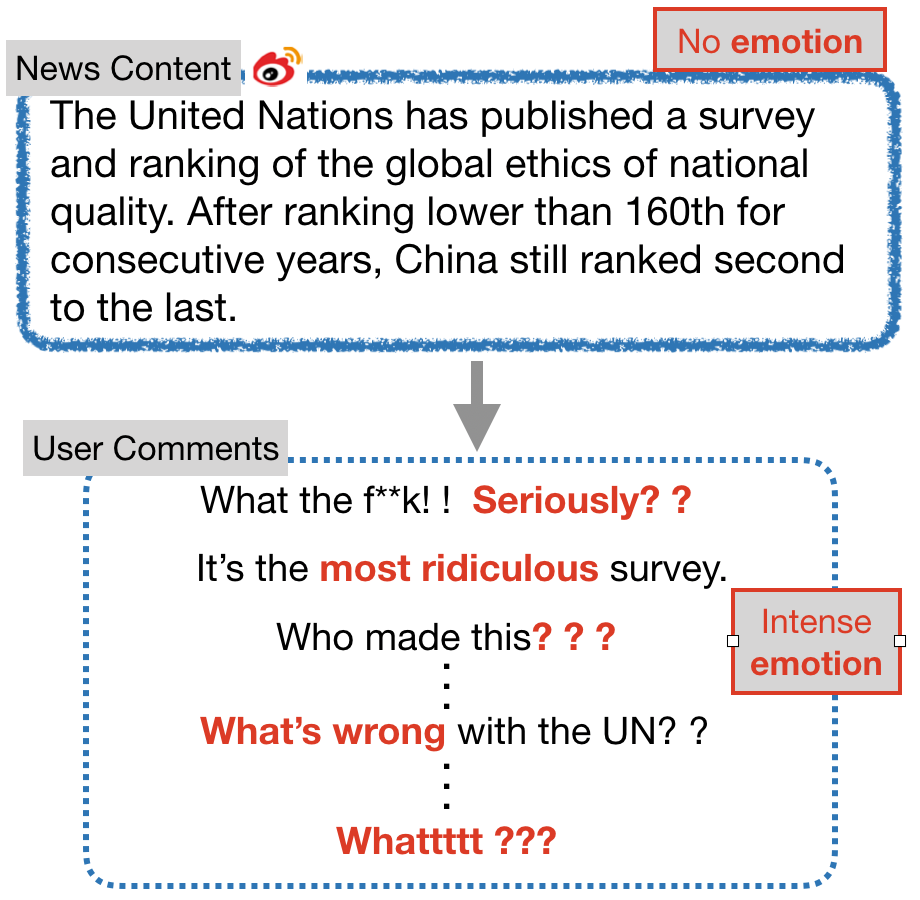
\includegraphics[width=1.65in]{./Figure/introcase2.png}}
		\end{minipage}
		\caption{Two fake news posts from Sina Weibo. (a) a post which contains emotions of astonishment and sadness in \textbf{news contents} that easily arouse the audience. (b) a post which contains no emotion, but raise emotions like doubt and anger in \textbf{user comments} by controversial topics.}
		\vspace{-0.3cm}
		\label{Fig:introcase}
	\end{figure}
	
	%\kai{In the next four paragraphs, the logic should be adjusted. The logic should be like: p2: describing existing work on fake news detection in a objective way, listing 2-3 representative work that you plan to compare in the experiments; p3: summarizing the limitations of existing work or propose your motivation clearly, such as the two scenarios you mentioned in Fig. 1., for each case, highlighting why it is helpful to detect fake newss. P4: summarizing the challenges and framework, and summarize the contributions}
	
	Existing works on fake news detection mainly focus on {\em news content} and {\em social context}. Feature-based classification models extract basic semantic and emotion features from content, and statistical features from users \cite{castillo2011information}. Propagation-based model construct the relationship network inside the event, and incorporate social conflicting viewpoint towards the event in the network \cite{jin2014news,jin2016news}. Recently, deep learning models are proposed to evaluate the credibility of information on social media, which deeply exploits the semantics information from news content\cite{ma2016detecting}. Basic social context features are fused into deep learning models in some studies\cite{guo2018rumor}. However, emotion information, which is crucial for fake news detection, is underutilized in these studies. Fewer studies leverage emotion in news contents and social context simultaneously for fake news detection.
	
	%However, existing works on fake news detection lack systematical and comprehensive exploration on emotion. Their attempts at utilizing emotion could be categorized to two clusters: 1) mining users' stances towards an event to evaluate the credibility of this event; and 2) extracting statistical emotional features and then incorporate these features in the whole feature sets or the model. Nevertheless, on the one hand, stance mining approaches mainly focus on the viewpoints of users, ignoring the reaction of the publisher which is a crucial indication of the event's credibility as well. And also, stance mining approaches are unable to capture emotions like {\em anxiety, anger, awe, etc}. On the other hand, extracting statistical emotional features highly rely on sentiment dictionaries, which is unreliable and inaccurate when applied on social media, because of the difference of word usage on social media and in real word. Problems such as emotion migration and minor coverage will happen while matching the words on social media with words in sentiment dictionary. Meanwhile, in these emotion feature works, weighted sum of sentiment words is too simple to measure sentiment metrics of a document.
	
	Fake news publishers often aim to spread information extensively and draw wide public attention. Longstanding social science studies demonstrate that the news which evokes high-arousal, or activating (awe, anger or anxiety) emotions is more viral on social media\cite{stieglitz2013emotions,ferrara2015quantifying}.  To achieve this goal, fake news publishers commonly adopt two approaches. First, publishers post news with intense emotions which trigger a high level of physiological arousal in the crowd. For example, in Figure \ref{Fig:introcase1}, the publisher uses rich emotional expressions (e.g., ``Oh my god!'') to make this information more impressive and striking. Second, publishers may present the news objectively to make it convincing whose content, however, is controversial which evoke intense emotion in the public, and finally spreads widely. As another example (see Figure \ref{Fig:introcase2}), the publisher writes the post in a unemotional way; while, the statement that China ranks second to the last suddenly bring on tension in the crowd, and people express their feeling of anger (e.g., ``most ridiculous''), shock and doubt (e.g., ``seriously?'') in comments.
	% 	and 2) present the news objectively to make it convincing whose content, however, is controversial which evoke intense emotion in the public, and finally spreads widely. Figure \ref{Fig:introcase1} demonstrates the first approach. The publisher uses rich emotional expressions to make this information more impressive and striking. While in Figure \ref{Fig:introcase2}, the publisher writes the post in a unemotional way. However, the statement that China ranks second to the last suddenly bring on tension in the crowd. People express their feeling of anger, shock and doubt in comments. 
	Therefore, learning emotion of the publisher and the users corporately has the potential to improve fake news detection performance.
	% , which is limited in majority of existing studies.
	
	To exploit emotion information for fake news detection, we first define two types of emotions: (1) \textbf{{\em publisher emotion}}: emotion of the publisher while posting information on social media; and (2) \textbf{{\em social emotion}}: emotion of users when the information disseminates on social media. 
	%In this paper, news content and user comments are used to capture {\em publisher emotion} and {\em social emotion} respectively.  
	In essence, we investigate: (i) how to capture signals of {\em publisher emotion} and {\em social emotion} from news content and user comments, respectively; (ii) how to exploit publisher and social emotions simultaneously for fake news detection. Our solutions to these two challenges results in a novel \underline{E}motion-based \underline{F}ake \underline{N}ews Detection framework ({\m}). Our main contributions are summarized as follows:
	%Firstly, we prove the difference of publisher emotion and social emotion between fake news and real news from various perspectives. A novel end-to-end \underline{E}motion-based \underline{F}ake \underline{N}ews Detection framework(EFN) is proposed which jointly learn the {\em publisher emotion} and {\em social emotion} by two modules: {\em content module} and {\em comment module}, and incorporate emotion with semantic information to detect fake news. 
	
	%Due to the limitations of sentiment dictionary based emotion representation, we leverage a emotion corpus on social media to obtain the emotion representation for each word, which is refereed as {\em emotion embedding} in this paper. To better fuse information from different source for each word or module, we design three {\em gates} which could selectively discard or maintain information from either source. 
	
	%The main contribution of this paper can be summarized as follows:
	\begin{itemize}
		
		\item We provide a principled way to capture the {\em publisher emotion} and {\em social emotion} signals, and demonstrate the importance of these two emotions from various perspectives on fake news detection.
		% 		\item We categorize the emotions on social media as {\em publisher emotion} and {\em social emotion}, and verify the importance of these two emotions on fake news detection.
		\item We propose a novel framework {\m}, which exploits a deep neural network to learn representations from {\em publisher emotion}, {\em social emotion} and content simultaneously, for fake news detection.
		% 		\item We propose a novel framework({\m}) to model the publisher emotion, social emotion and content simultaneously, which can learn emotion
		% 		where {\em emotion embedding} is adopted for better emotion representation and gate mechanism is applied for fusion.
		\item We conduct experiments on real world datasets to show the effectiveness of {\m} for fake news detection. 
		%The result shows that our framework outperforms the existing feature-based methods and state-of-art neural network models.
	\end{itemize}
	
	
	\section{Related Work}
	% In this section, we briefly review the work related to our proposed framework. Specifically, we mainly focus on three topics: rumor detection, emotion representation, gate mechanism.
	
	We briefly describe the related work from three-folds: i) Fake News Detection; ii) Emotion Representation; and iii) Multi-modal Fusion.
	
	\subsection{Fake News Detection}
	%\kai{Change to fake news}
	%Most of existing studies defined rumor detection task as a classification task. And typically, they could be categorized into three paradigms: hand-crafted feature based approaches, propagation-based approaches, and neural network approaches. 
	Previous fake news detection studies mostly focus on extracting features and training a classifier to predict the credibility of news. \cite{castillo2011information} manually extracts a wide range of features including user features, content features, propagation features and topic features. \cite{yang2012automatic} demonstrates the effectiveness of location and client; Besides feature-based models, propagation-based approaches aim to mine the relations between various entities in a event. \cite{gupta2012evaluating} firstly introduces propagation network in credibility evaluation by constructing a relation network. \cite{jin2014news,jin2016news} applies similar hierarchical structure on microblogs which consists of news, sub-events and messages. Recently, neural network models are adopted for fake news detection. \cite{ma2016detecting} firstly applies RNN for fake news detection on social media, modeling the posts in a event as a sequential time series. \cite{guo2018rumor} proposes a social attention network to capture the hierarchical characteristic of events on microblogs. 
	
	So far,  emotion in these works is used as either emotion feature sets or viewpoints of users, which requires more systematical and comprehensive explorations in future work.
	
	\subsection{Emotion Representation}
	
	Early studies primarily use hand-crafted features for representing emotion of text, which highly rely on sentiment dictionaries. There are several widely-used emotion dictionaries, including WordNet \cite{wordnet} and MPQA \cite{MPQA}for English, and HowNet~\footnote{http://www.keenage.com/html/e\_index.html} for Chinese. However, this method may encounter problems of emotion migration and low coverage on social media, because of the differences of word usage on social media and in real word. 
	
	Learning task-specific emotion embedding with neural network has been prove to be effective. \cite{Tang14} leverage a dataset of tweets to obtain emotion embedding. \cite{agrawal2018learning} learns emotion-enriched word-representation on product reviews, with a much smaller corpus. This method could be easily applied on social media by using online emotion corpus, which could largely overcome the limitations of sentiment dictionaries.
	
	\subsection{Multimodal Fusion}
	The simplest approach is concatenation, which fuses different modality vectors by concatenation. \cite{silberer2017visually} employ a stacked autoencoder to learn multimodal representations by embedding linguistic and visual inputs into a common space. However, these methods treat the different modalities equally in fusion. In \cite{jin2017multimodal}, the authors employ the high-level representation of visual modal as the external attention vector to weigh the components of textual modality. Gate mechanism is also widely used in many fusion work. LSTM \cite{hochreiter1997long} and GRU \cite{bahdanau2014neural} tackle the long-term dependency problems of RNN with different gates that could control how information from last time step and current inputs updates at current unit, which is another form of fusion. \cite{wang2018learning} deploys gates to learn the weights of different modality representations for each word. 
	
	Considering the importance of emotion in fake news detection, we proposed a novel fake news detection framework which could exploit emotion information from the publisher and users with the help of emotion embedding and gates.
	
	% \section{Emotion Exploration on Rumor}
	\section{A Preliminary Analysis on Emotion Signals }
	
	% In this section, we explore the contrast of Emotion Categories, Emotional Intensity and Emotional Vocabulary Expression between fake news and Non-Rumor. The analyzed data in this Section is same to our experiments dataset of Section 4.6. It contains 7880 fake news, 7907 Non-Rumor and their respective comments, which are about 160,000 altogether (Details about the data will be described in Section 4.6). And the result of analysis verifies the importance of mining emotion on fake news Detection.
	
	To explore the relationships between emotions and fake news on social media, we perform a preliminary data analysis on emotions signals for fake and real news in news content and user comments respectively. We collect the datasets from a popular microblog platform Weibo~\footnote{www.weibo.com} (details of data preparation are introduced in Sec~\ref{sec:data}). We have collected 7,880 fake news pieces and 7,907 real news pieces, and their related user comments on Weibo. The analysis is performed from three perspectives: 1) the emotional category; 2) the emotional intensity; and 3) the emotional expression.
	
	\subsection{Emotional Category}
	%\kai{Use 1-2 sentences to explain WHY emotion categories are compared here}
	Generally, fake news is sensational and inflammatory. It could arouse specific kinds of emotion among the users, such as suspicion, anxiety or shock. Therefore, we select 5 fine-grained emotion categories to investigate emotions in fake news and real news, including \textit{anger}, \textit{sadness}, \textit{doubt}, \textit{happiness} and \textit{none} (Some contents may not contain emotional information). We adopt the emotion classifier in Sec~\ref{sec:classifier} to annotate our experimental data with emotion categories. 
	
	Figure \ref{Fig:ec1} and \ref{Fig:ec2} exhibit the distribution of emotion categories in news content and user comments respectively. In fake news' content, the proportion of \textit{anger} is 9\% higher than it in real news’, while the percentage of \textit{happiness} is 8\% lower. Same trend happens in the user comments. In addition, the proportion of sadness in fake news' contents and doubt in fake news' comments is much higher than them in real news.  The result demonstrates that, compared to in real news, both the publisher and users tend to express more high-arousal emotions, such as anger, sadness and doubt in fake news.
	
	\begin{figure}[h]
		\centering
		
		%大图:0.44,3.25in
		\begin{minipage}[t]{0.23\textwidth}
			\subfloat[News Content]{\label{Fig:ec1}%%
				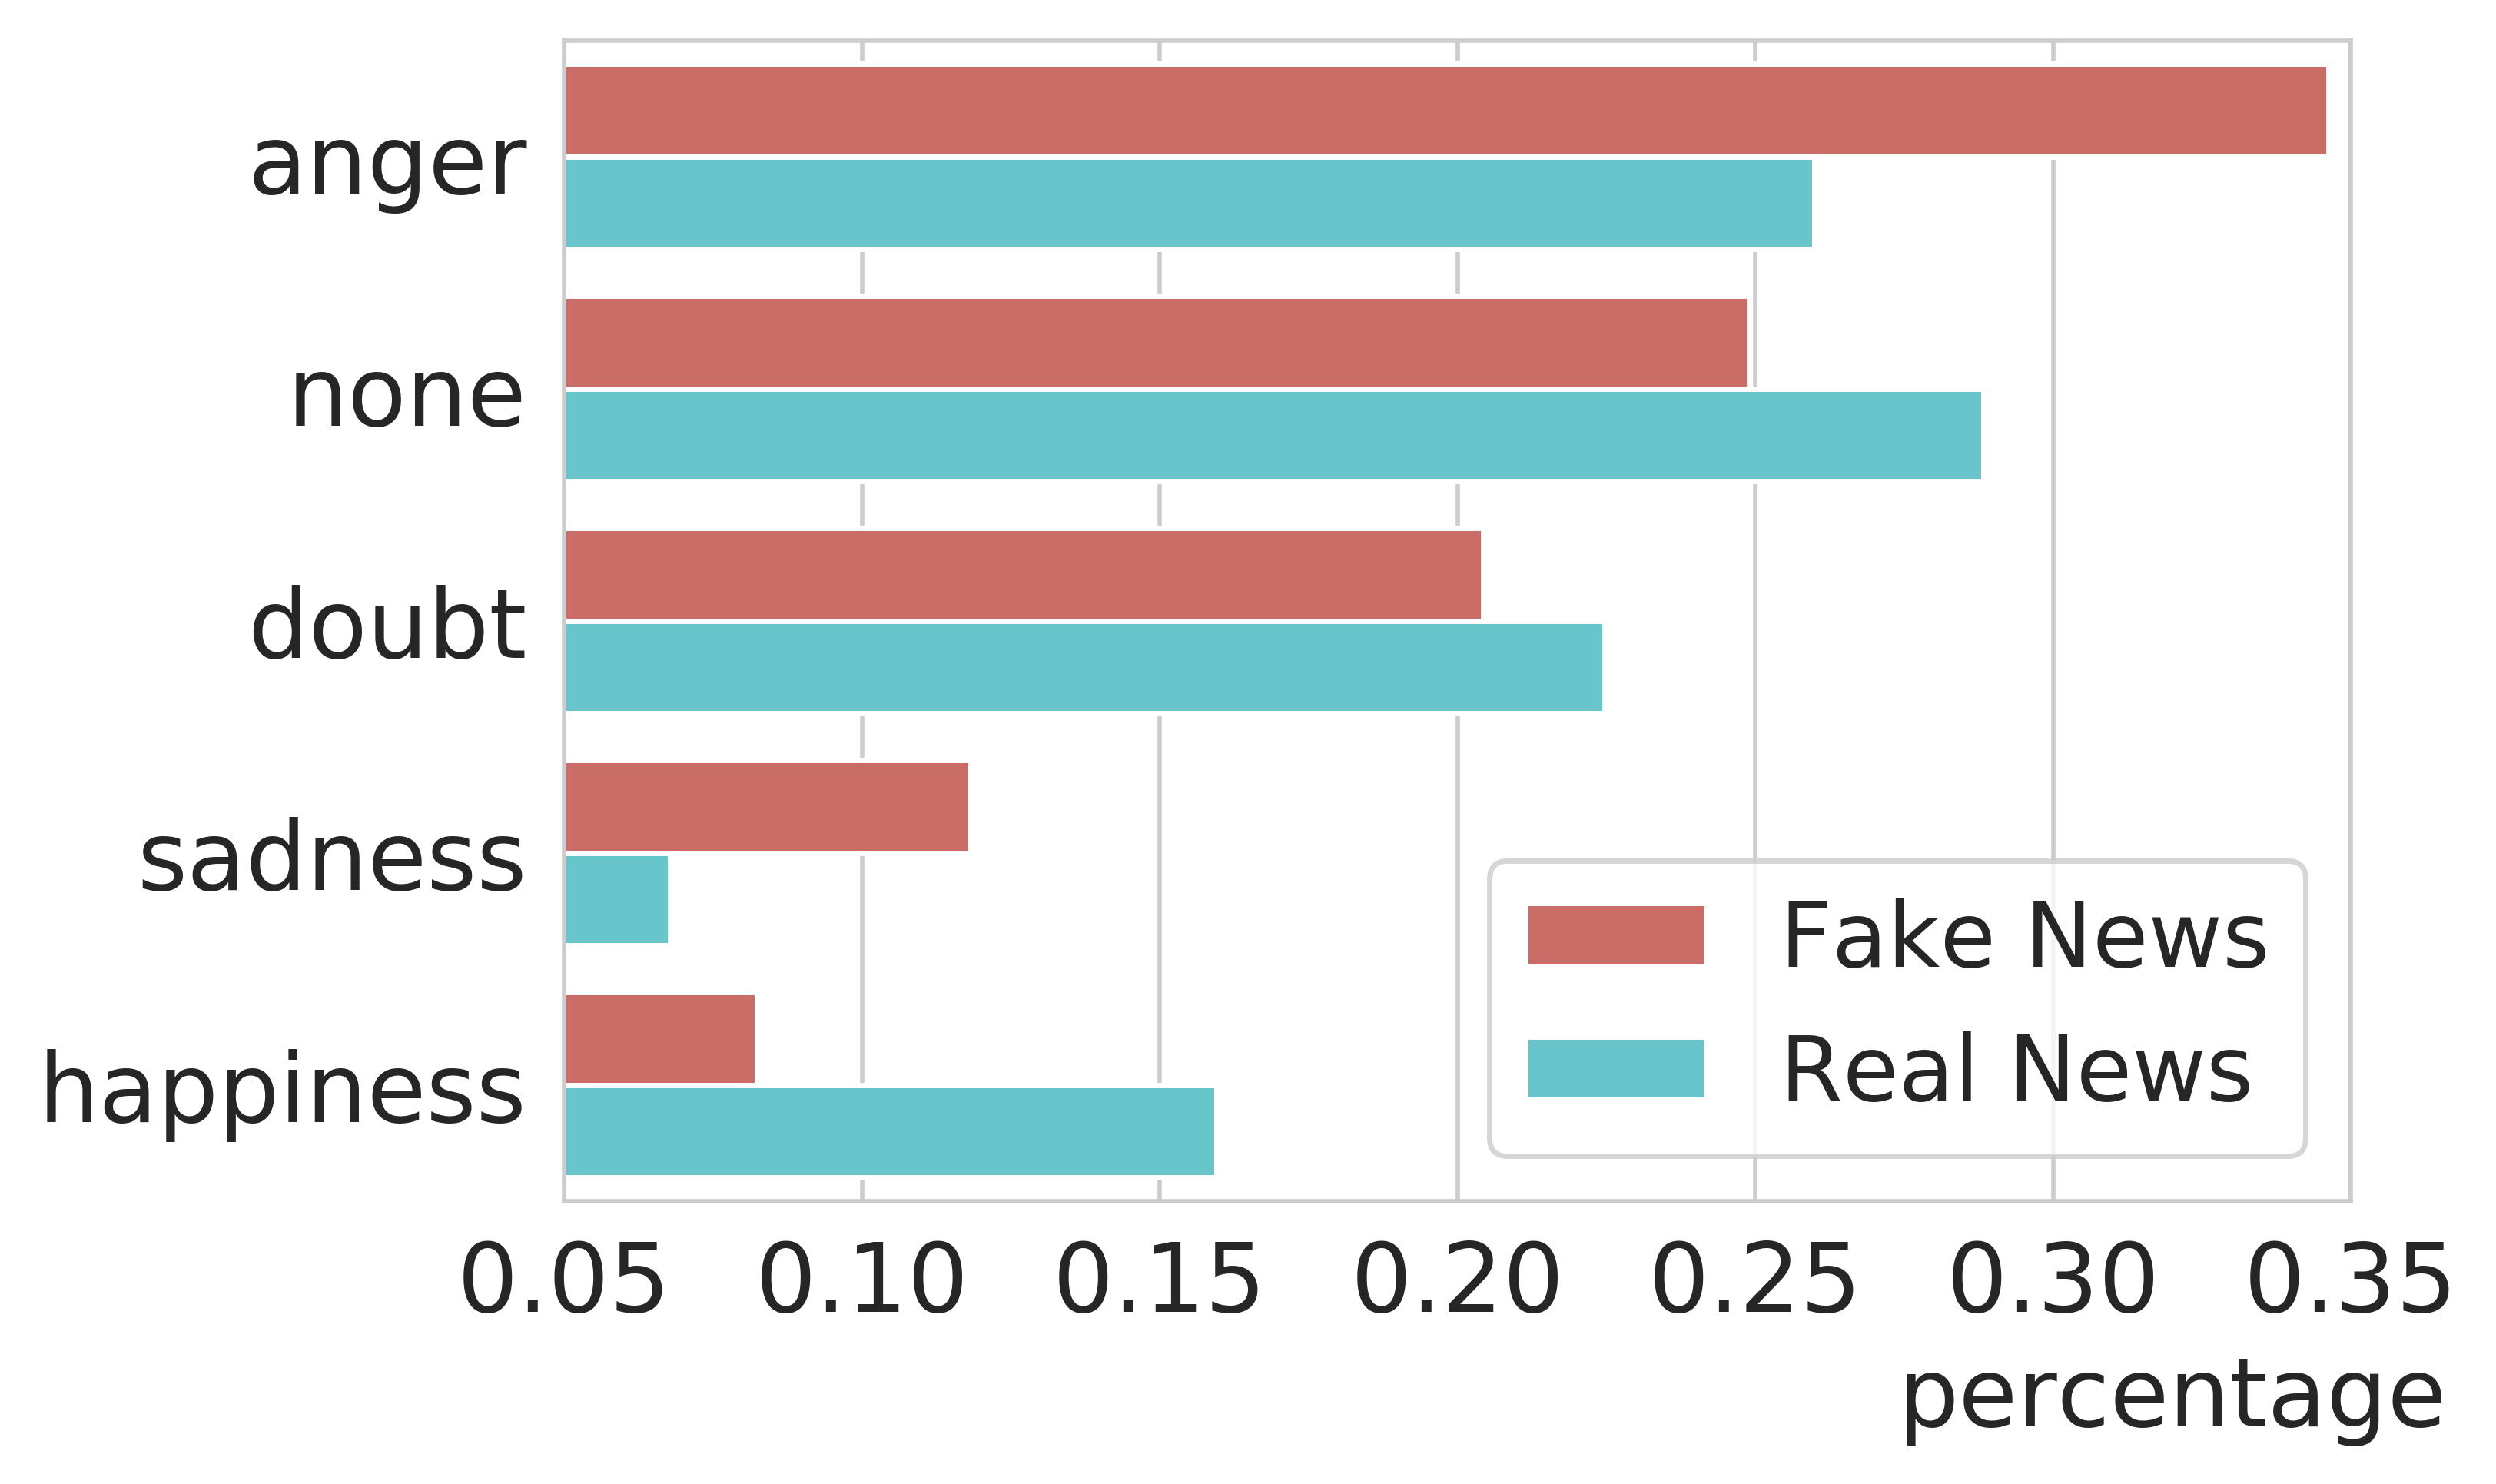
\includegraphics[width=1.68in]{./Figure/emotion-category-main.png}}
		\end{minipage}
		\begin{minipage}[t]{0.23\textwidth}
			\subfloat[User Comments]{\label{Fig:ec2}%%
				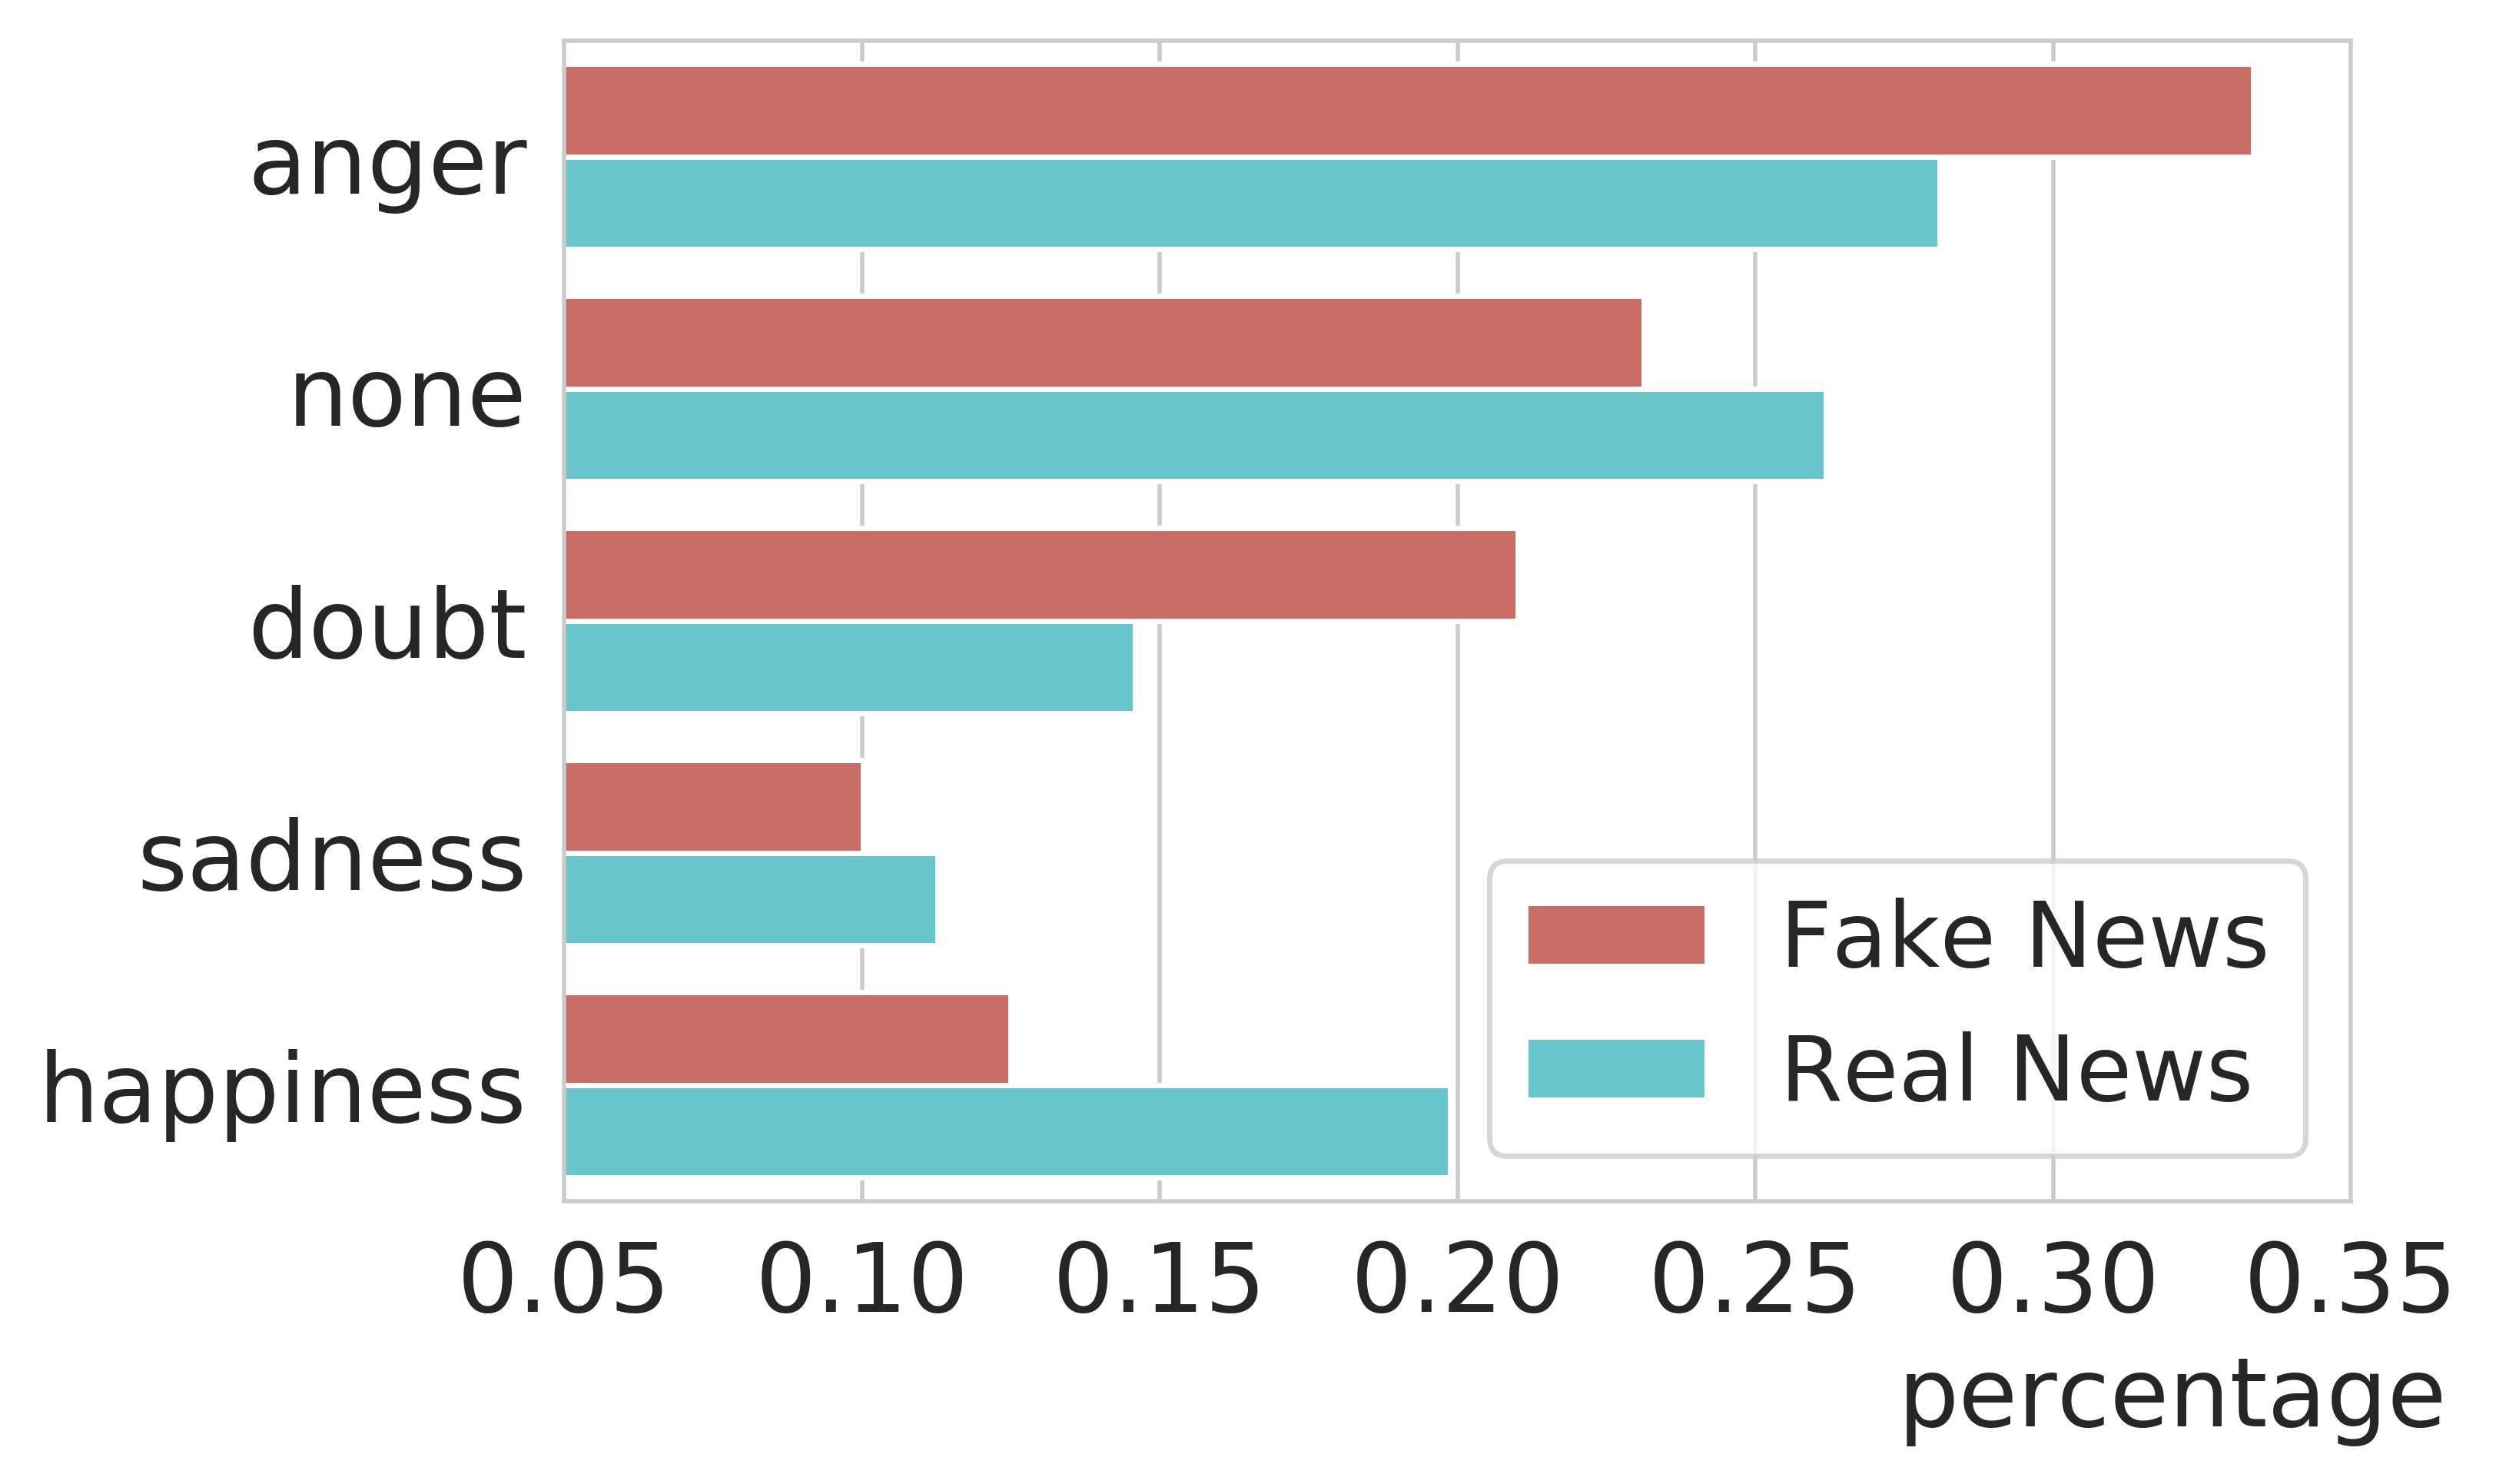
\includegraphics[width=1.68in]{./Figure/emotion-category-comments.png}}
		\end{minipage}
		
		\caption{Distributions of emotional category of fake news and real news in: (a) news content and (b) user comments. {\em Anger} is more likely to appear in fake news, while real news arouse more {\em happy} emotion in both sources}
		\vspace{-0.3cm}
		\label{Fig:emotionCategories}
	\end{figure}
	
	\subsection{Emotional Intensity}
	%\kai{Use 1-2 sentences to explain WHY emotion intensity are compared here; add one sentence to explain what is emotion intensity}
	%According to our assumption, the content emotion of rumor events and their emotion evoked in crowds, which we define as social emotion, tend to be quite intense to impress the audience and spread extensively. Hence we explore the emotional intensity of rumor to make it solid.
	
	Each document also owns an emotional intensity level in each emotional category. For example, the intensity of {\em I'm super happy} is much stronger than intensity of {\em I'm happy} in happiness emotional category. Fake news is expected to express negative emotion with stronger intensity which could further arouse the intense emotions in the public. In this section, we take the output probability of emotion classifier model’s softmax layer as the emotional intensity level for each emotional category, which is a continuous value between 0 and 1.
	
	In Figure \ref{Fig:emotionalIntensity}, we can see that, regardless of sources, the emotions of \textit{anger}, \textit{sadness} and \textit{doubt} in fake news are much more severe than in real news. And this discrepancy is more drastic in news content. In conclusion, both the publisher and users are more possible to express stronger negative emotions in fake news than in real news, while the trend of positive emotion is reverse.
	
	\begin{figure}[h]
		\centering
		
		% 大图:0.44,2.75in
		\begin{minipage}[t]{0.23\textwidth}
			\subfloat[News Content]{\label{Fig:ei1}%%
				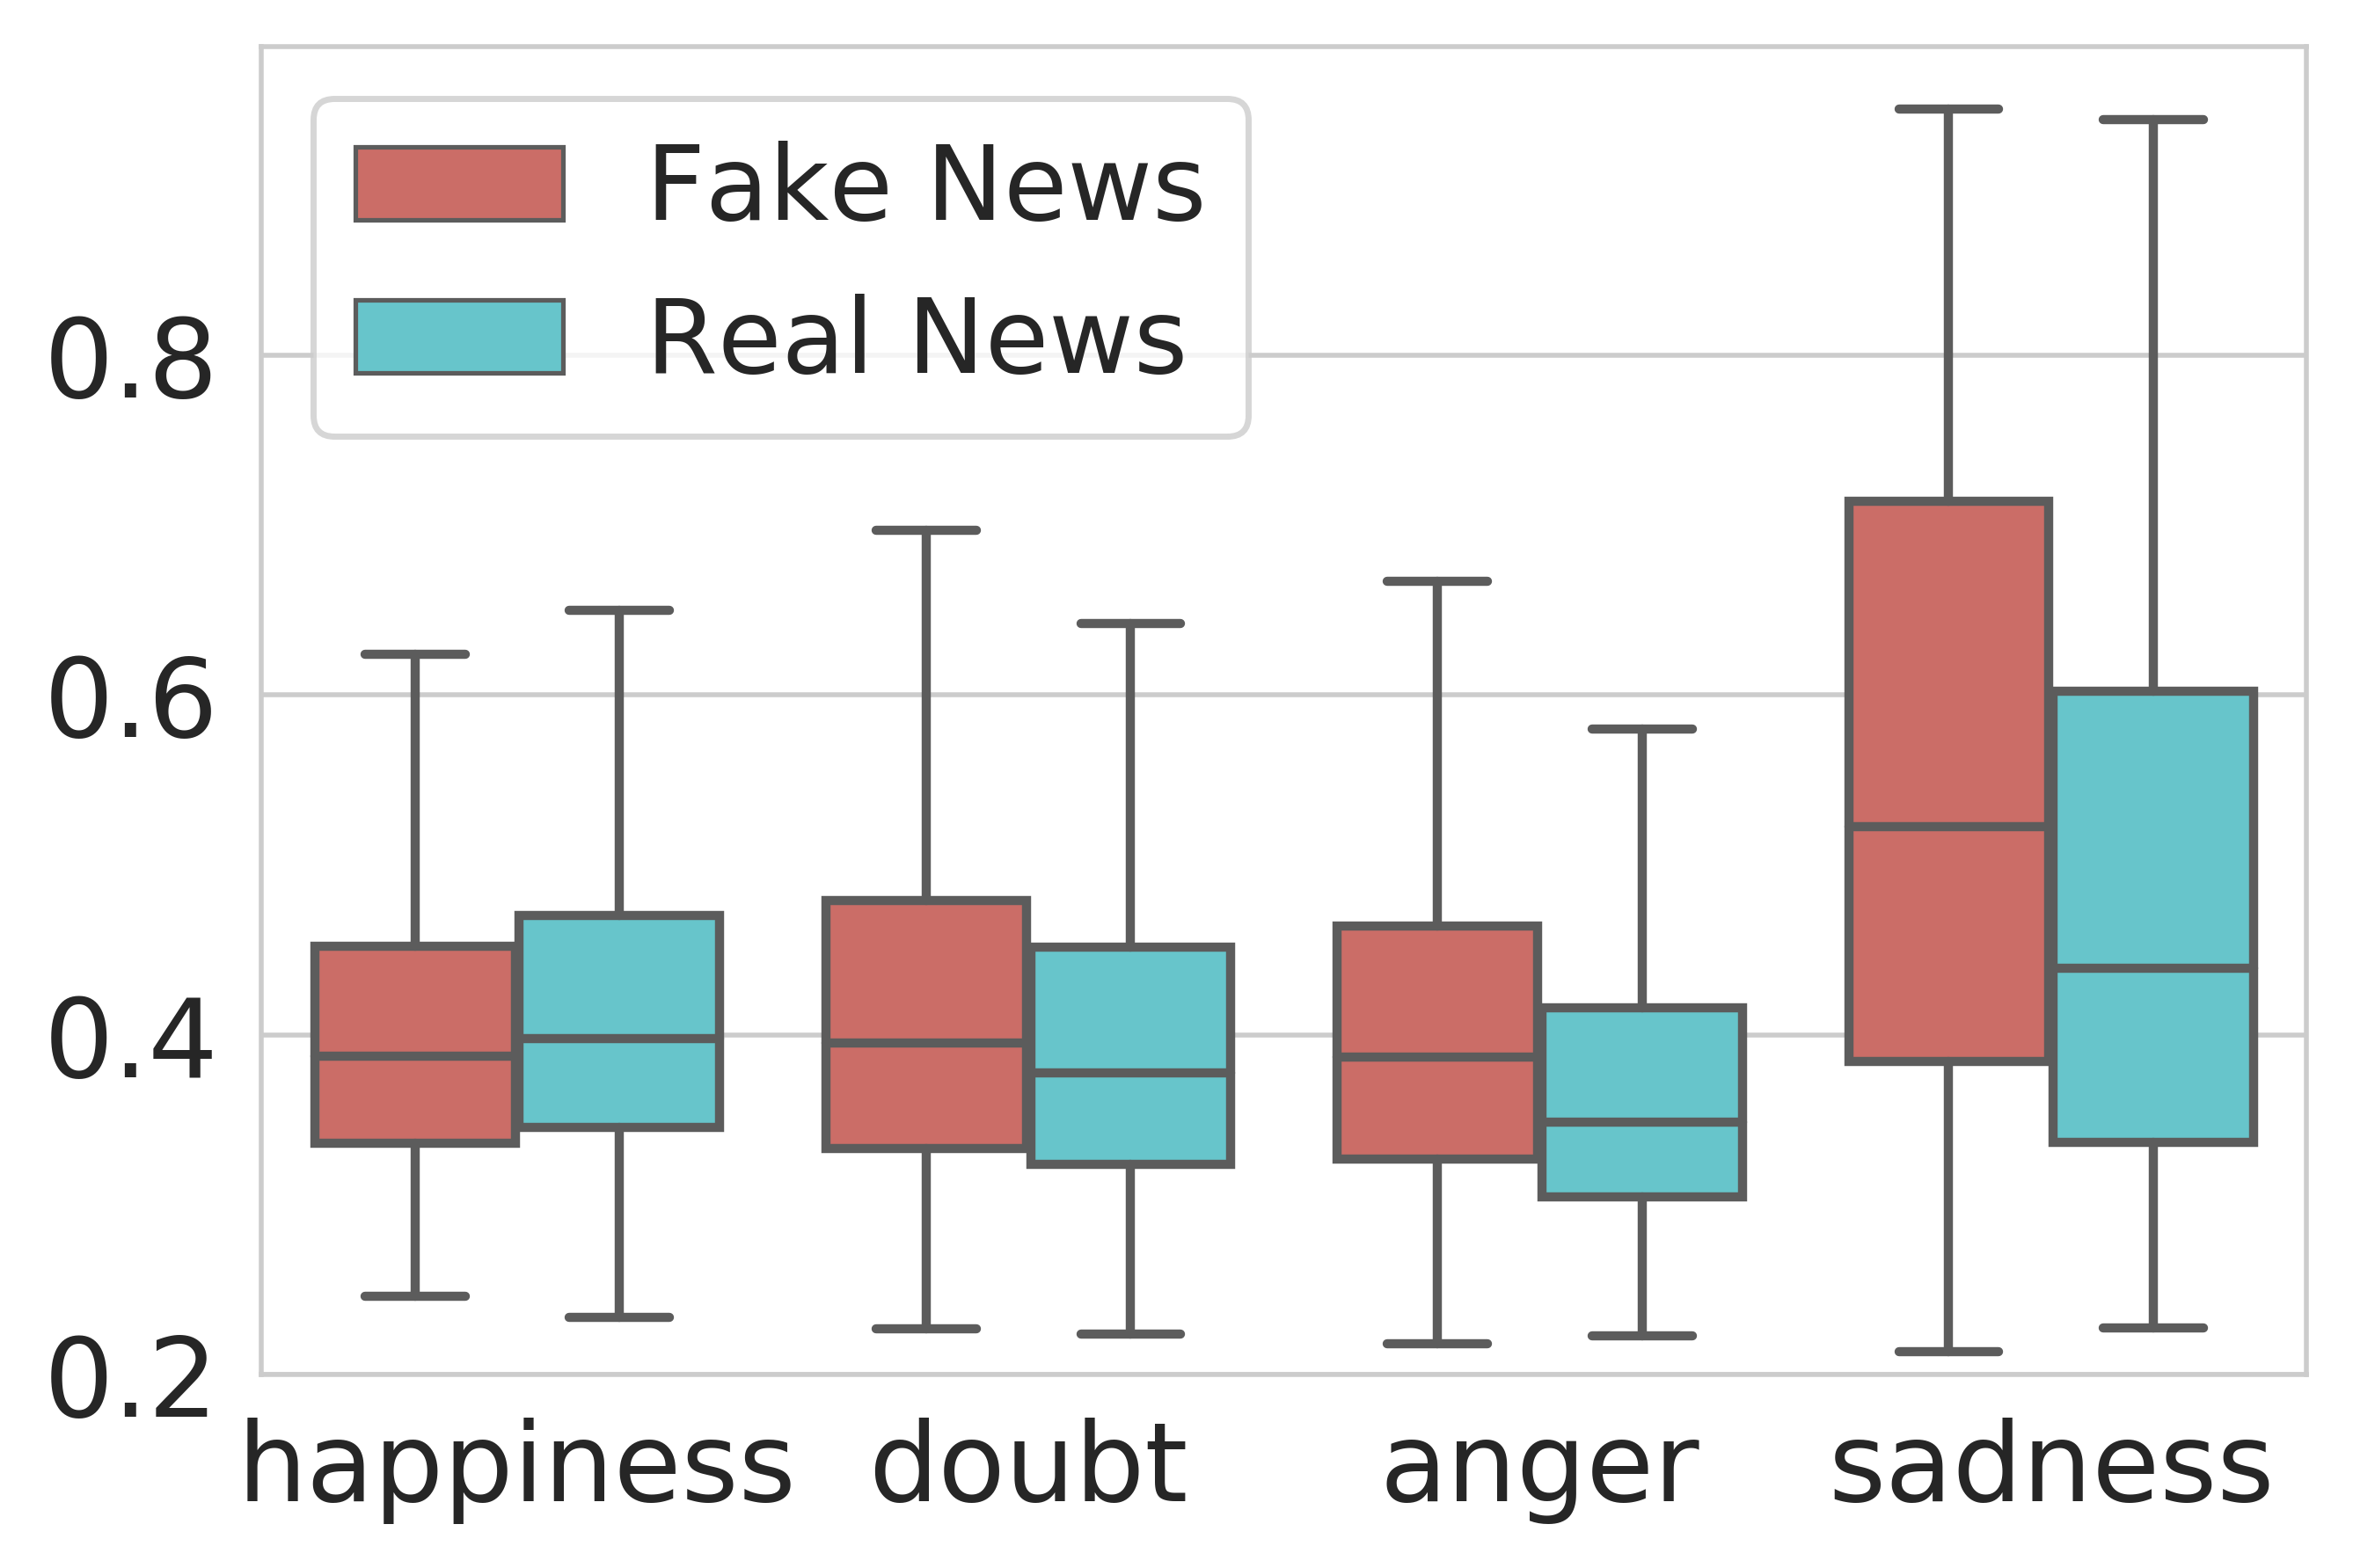
\includegraphics[width=1.65in]{./Figure/emotion-intensity-main.png}}
		\end{minipage}
		\begin{minipage}[t]{0.23\textwidth}
			\subfloat[User Comments]{\label{Fig:ei2}%%
				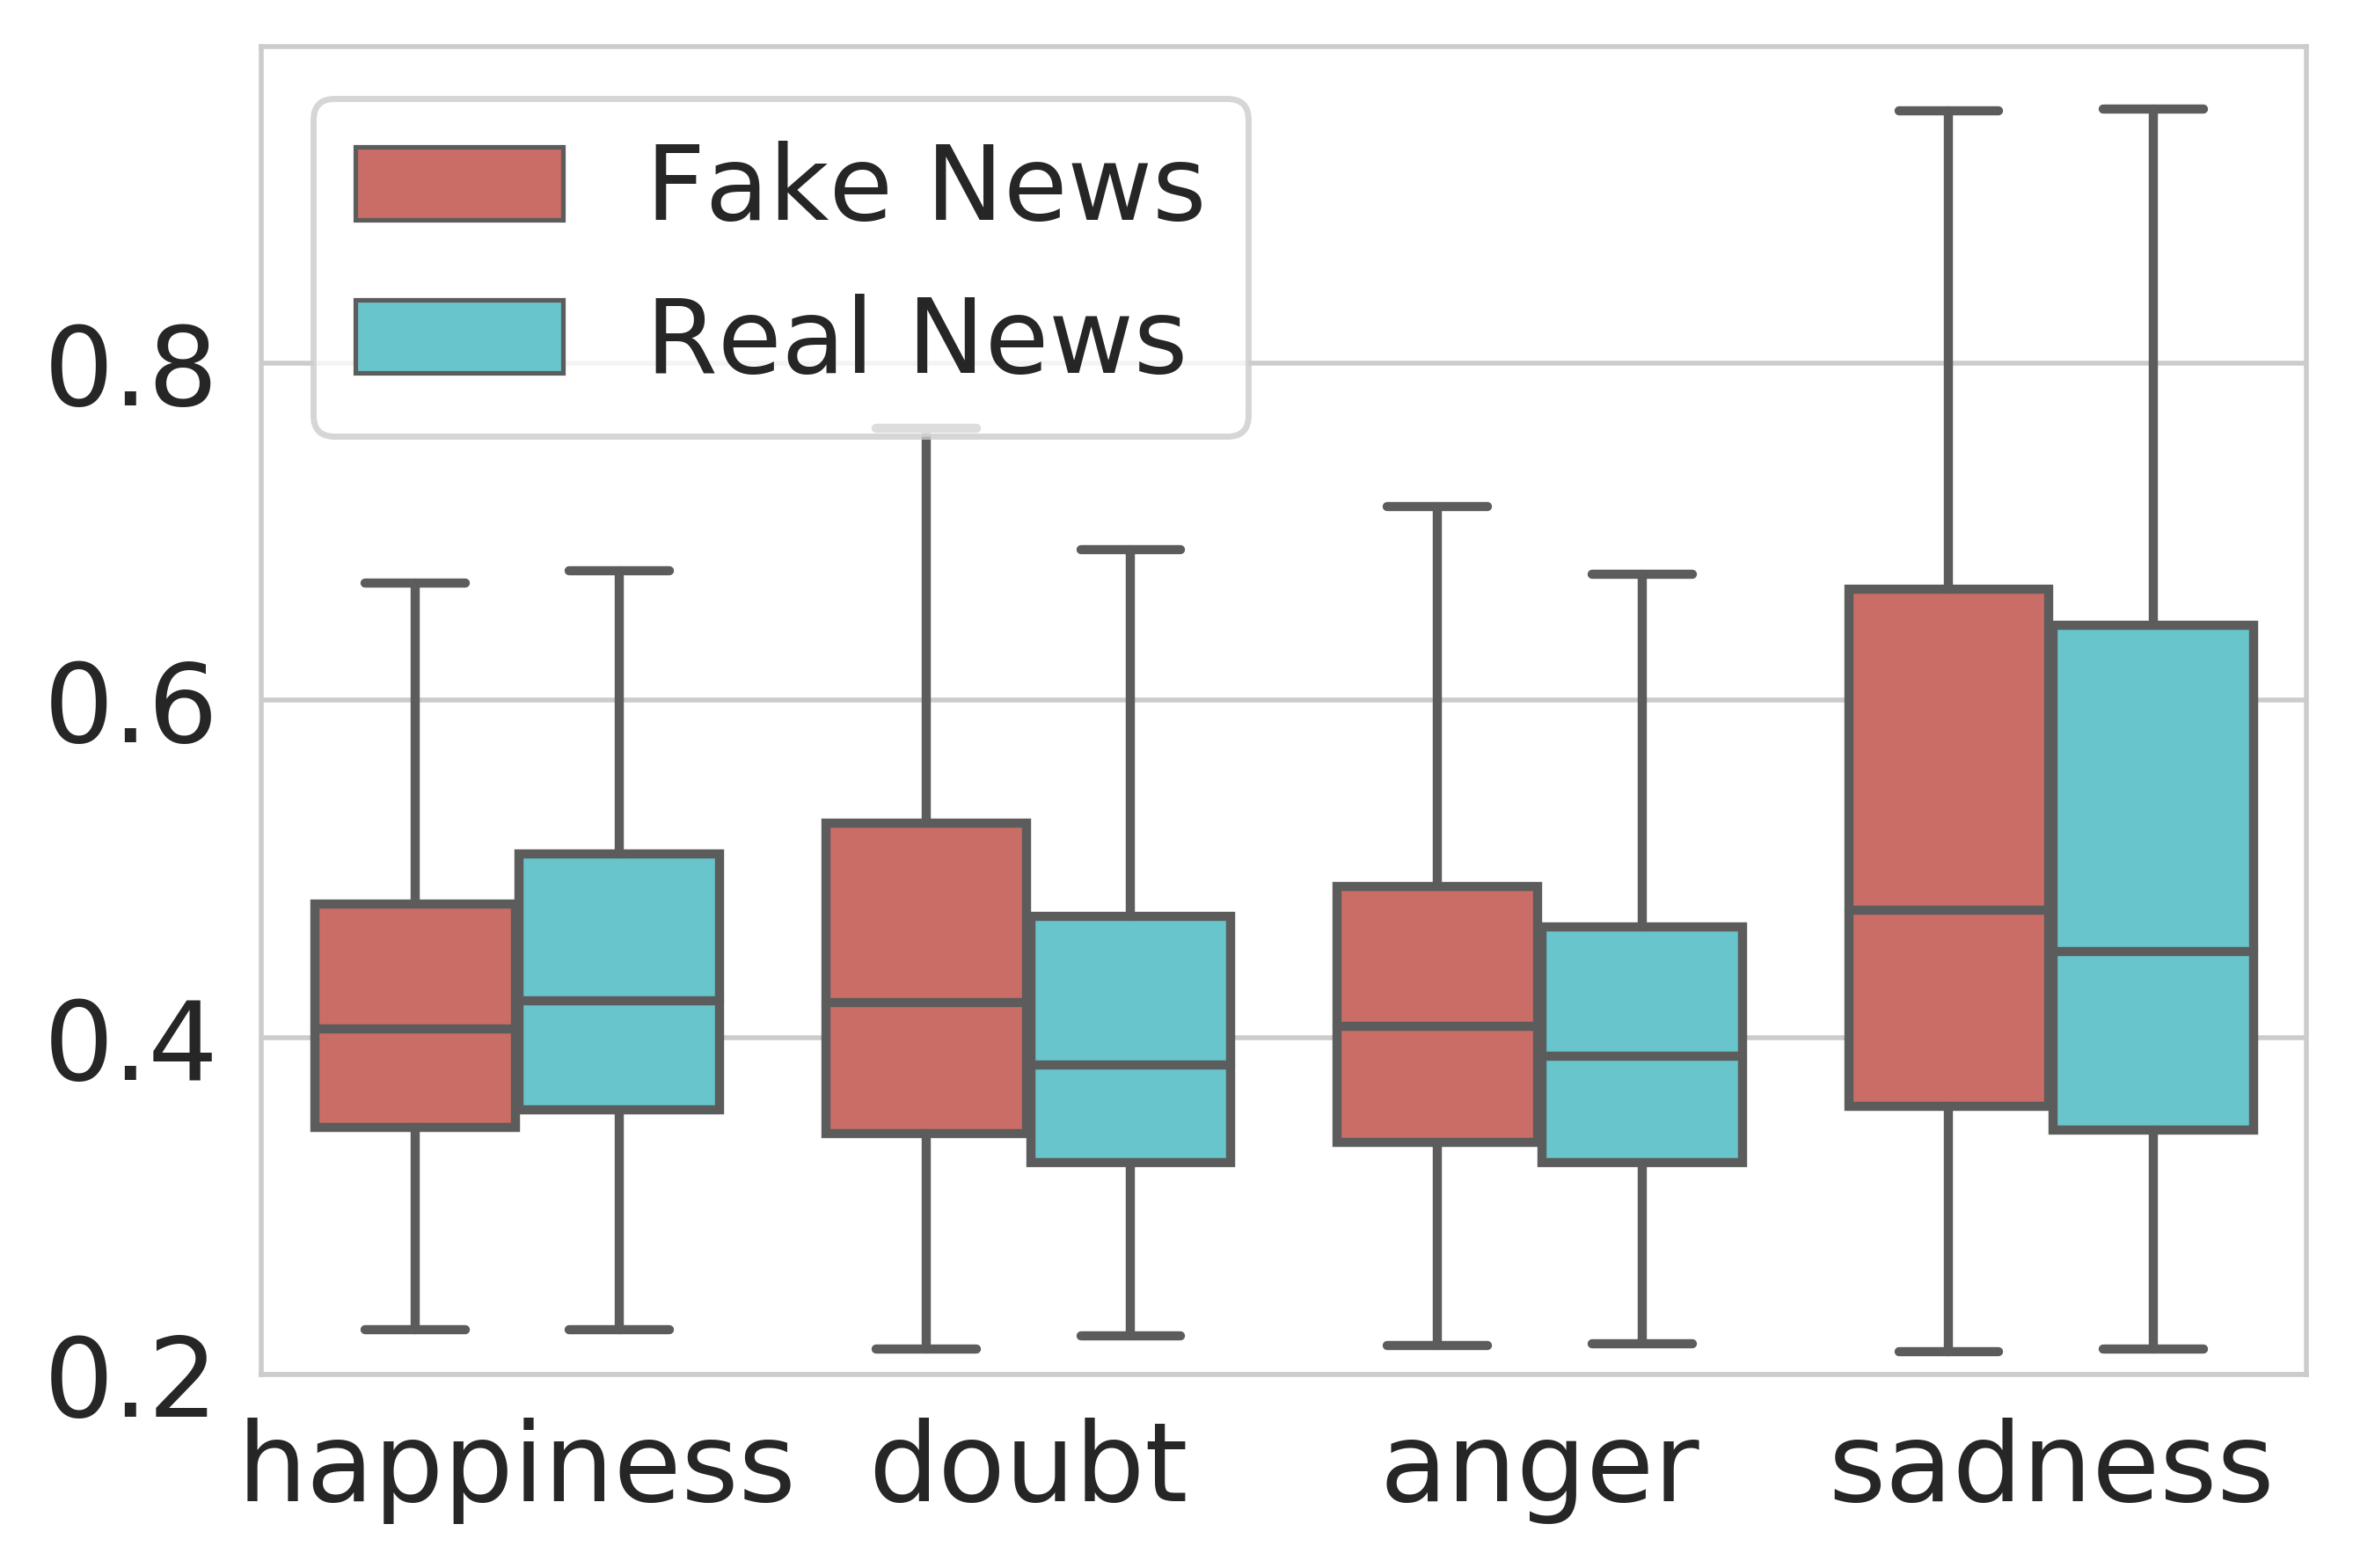
\includegraphics[width=1.65in]{./Figure/emotion-intensity-comments.png}}
		\end{minipage}
		
		\caption{Distributions of emotional intensities level of fake news and real news in: (a) news content and (b) user comments. The intensities of emotion \textit{anger}, \textit{sadness} and \textit{doubt} in fake news are all stronger than in real news.}
		\label{Fig:emotionalIntensity}
		\vspace{-0.3cm}
	\end{figure}
	
	\subsection{Emotional Expression}
	%\kai{Use 1-2 sentences to explain WHY emotion expression are compared here}
	%The analysis above has revealed that the distributions of emotion categories of fake news and Non-Rumor gap a lot. Moreover, we extract the differences of emotional vocabulary expression between the two for same kinds of emotion.
	
	Different people may express their moods with different linguistic usage. For example, some people like using plain words to express their feelings, while others prefer exaggerated words. In fake news, inciting words might be more preferred due to the controversial news content. To analyze the differences of emotional expression, we extract the top-weighted words for expressing {\em anger} in real news and fake news respectively. We adopt the widely-used method in \cite{nlpcc14} to calculate the weight of each word in the dataset for expressing specific kinds of emotion. 
	%The weights is positively correlated with the word's frequency in this emotion category, and negatively correlated with its frequency in other emotion categories and in the whole dataset. 
	%In practice, we mix the top words in news content with their comment, because the their top words are similar. 
	The top-weighted 30 words in fake news and real news are shown in Figure \ref{Fig:emotionalExpression}. 
	\begin{figure}[h]
		\centering
		
		\begin{minipage}[t]{0.23\textwidth}
			\subfloat[Fake News]{\label{Fig:ee1}%%
				\includegraphics[width=1.6in]{./Figure/words-rumor-anger.png}}
		\end{minipage}
		\begin{minipage}[t]{0.23\textwidth}
			\subfloat[Real News]{\label{Fig:ee2}%%
				\includegraphics[width=1.6in]{./Figure/words-truth-anger.png}}
		\end{minipage}
		
		\caption{Emotional expressions for \textit{anger} in fake news and real news. Compared to real news, fake news use more fierce and extreme words to express {\em anger}.}
		\vspace{-0.2cm}
		\label{Fig:emotionalExpression}
	\end{figure}
	
	We can see that fake news conveys \textit{angry} with much more fierce and extreme words like {\em "damn it", "scum"}. Similar circumstance also exists in other negative emotional categories. Therefore, people use different words for emotional expression in fake and real news.
	
	In summary, we make the following conclusions from these experiments: i) both the publishers and users are more likely to spread more negative emotions in fake news than in real news; ii) participants of fake news tend to express negative emotions with stronger intensities; iii) while expressing a specific kind of emotion, people in fake news prefer exaggerated and inflammatory words. 
	%Therefore, exploiting emotion would be great helpful for detecting fake news on social media.
	
	\section{Modeling Emotions for Fake News Detection}
	
	In this section, we present the details of the proposed end-to-end emotion based fake news detection framework {\m}. It consists of three major components (see Figure~\ref{Fig:framework}): i) the content module mines the information from the publisher, including semantic and emotions information in news contents; and ii) the comment module captures semantic and emotion information from users; and ii) the fake news prediction component fuses the high-level features from both news content and user comments and predict fake news. 
	% 	The whole framework is trained end-to-end.
	
	\subsection{Content  Module}
	News contents contain the cues to differentiate fake and real news. We have shown that the distributions of emotion categories are different for fake and real news pieces, which demonstrate the potential to use news content emotions to help detect fake news. 
	
	% Content module in this paper aim to learn the information from the publisher, especially the semantic information and emotion information of the source posts. Figure \ref{Fig:contentmodule} demonstrate the structures of content module. We employ bidirectional gated recurrent unit network(BiGRU)\cite{bahdanau2014neural} to learn the high-level representation of semantic and emotion, and even the content module. GRU is a refined recurrent neural network which is proposed by \cite{bahdanau2014neural}, where the reset gate $r_t$ and update gate $z_t$ together control how information is updated to the state. Bidirectional structure enable each state to capture information from both previous and subsequent context information. BiGRU has been widely applied in many natural language processing tasks, such as text classification, machine translation, question answering, etc. And a gate {\em gateT} is used on each word, transferring the three inputs: emotion embedding, word embedding and sentence emotion features to a new low dimensional continuous vector. 
	
	% In detail, each word would be represented as two embedding vector, one is word embedding and another is emotion embedding. The word embedding vector for each word is initialized with the pre-trained word2vec\cite{mikolov2013distributed} on a given datasets. And the emotion embedding is initialized with the embedding vectors which is extracted from the embedding layers that described in section 4.1. Let $ P = \{p_1, ...,p_N\}$ denote the source posts in the datasets. And let $T = \{t_1, ...t_M\}$ be the words of a post, where $t_i$ represent $i$-th word in this post. Their corresponding emotion embedding and word embedding representation are $T_e = \{t_1^e, ...,t_M^e, t_i^e \in \mathbb{R}^k\} $ and $T_w = \{t_1^w, ..., t_M^w, t_i^w \in \mathbb{R}^l\}$, as the dimensions of emotion embedding and word embedding vectors are $k$ and $l$ respectively.
	\begin{figure}[t]
		\centering
		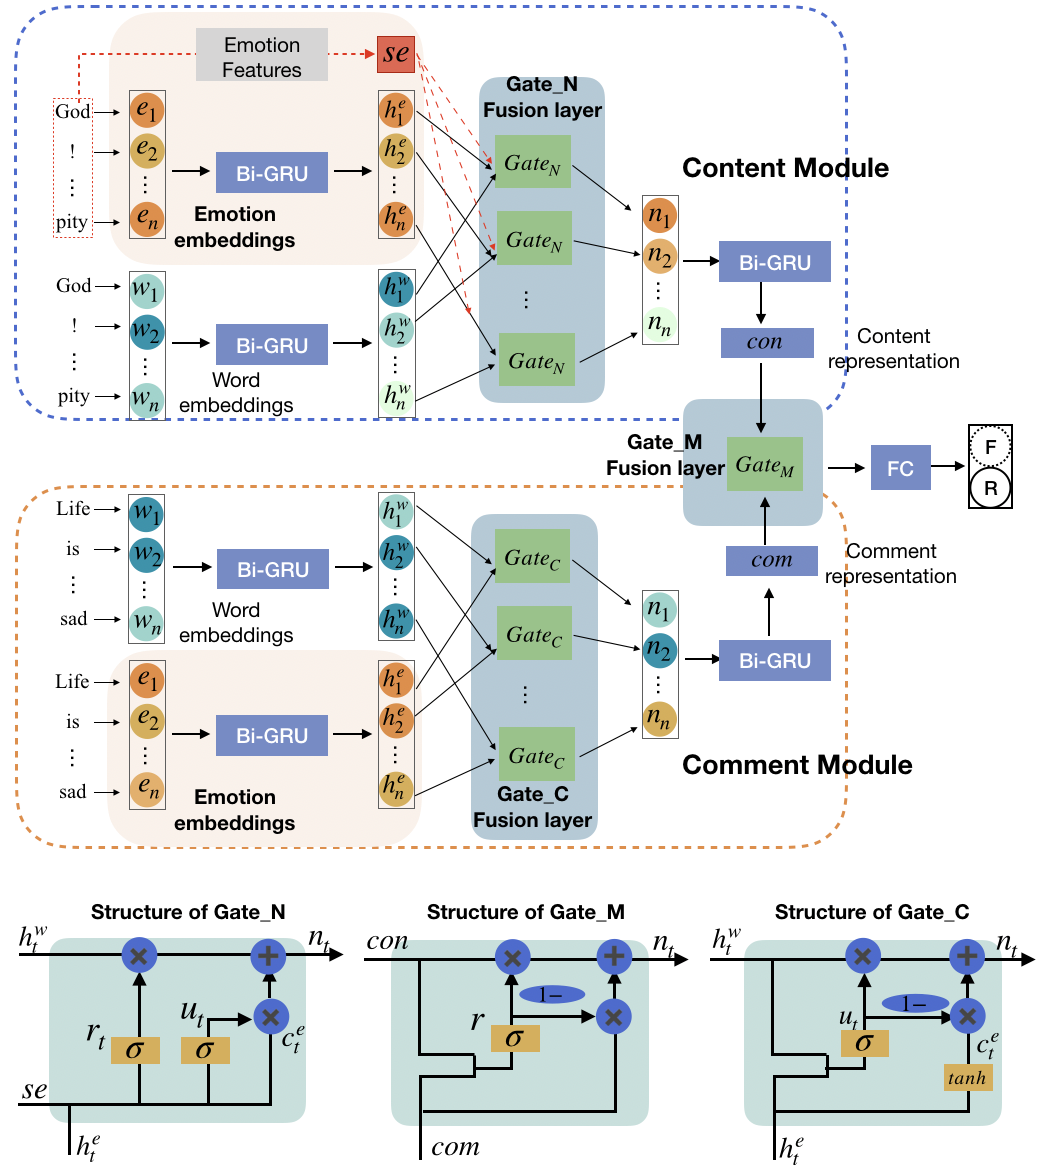
\includegraphics[width=0.5\textwidth]{./Figure/framework.png}
		\caption{The proposed framework {\m} consists of three components: (1) the news content module; (2) the user comments module, and (3) the fake news prediction component. The previous two modules are used to model semantics and emotions from the publisher and users respectively, while prediction part fuse information of these two module and make prediction. Three gates at the bottom are used for multimodal fusion in different layers.}
		\label{Fig:framework}
		\vspace{-0.3cm}
	\end{figure}
	\paragraph{Word Encoder}
	We learn the basic textual feature representations through a recurrent neural network (RNN) based word encoder. Though in theory, RNN is able to capture long-term dependency, in practice, the old memory will fade away as the sequence becomes longer. To make it easier for RNNs to capture long-term dependencies,
	Gated recurrent units (GRU)~\cite{bahdanau2014neural} is designed in a manner to have more persistent memory. To further capture the contextual information of annotations, we use bidirectional GRU to model word sequences
	from both directions of words. For each word $t_i$, the word embedding vector $t_i^w$ is initialized with the pre-trained word2vec\cite{mikolov2013distributed}. The bidirectional GRU contains the forward GRU $\overrightarrow{f}$ which reads each sentence from word $t_0$ to $t_M$ and a backward GRU $\overleftarrow{f}$ which reads the sentence from word $t_M$ to $t_0$:
	
	% Each sentence in the news source post could be represented as a word embedding matrix by sequentially concatenating the word embedding vectors. We firstly use a bidirectional GRU\cite{bahdanau2014neural} to encode each word to a higher level representation, by summarizing contextual information from both directions for words. The bidirectional GRU contains the forward GRU and backward GRU:
	\begin{equation}
	\begin{aligned}
	\overrightarrow{h_i^w} = \overrightarrow{GRU}(t_i^w), i \in [0, M],\\
	\overleftarrow{h_i^w} = \overleftarrow{GRU}(t_i^w), i\in [0, M].
	\end{aligned}
	\end{equation}%
	for a given word $t_i$, we could obtain its word encoding vector $h_i^w$ by concatenating the forward hidden state $\overrightarrow{h_i^w}$ and backward hidden state $\overleftarrow{h_i^w}$, i.e., $h_i^w=[\overrightarrow{h_i^w}, \overleftarrow{h_i^w}]$
	
	\paragraph{Emotion Encoder}\label{sec:classifier}
	Similar to the word encoder, we adopt bidirectional GRU to model the emotion feature representations for the words. To preserve the emotion signal for each word, we first introduce how to obtain an emotion embedding vector $t_i^e$ for each word $t_i$.
	
	Inspired by recent advancements on deep learning for emotion modeling~\cite{agrawal2018learning}, we train a recurrent neural network to learn the emotion embedding vectors. Following traditional settings~\cite{hu2013unsupervised}, we first obtain a large-scale Weibo datasets that contain emoticons, and use the emoticons as the emotion labels. We initialize words with one-hot vectors instead of word2vecs for not learning too much semantics. After initiation, all word vectors pass an embedding layer which project each word from the original one-hot space into a low dimensional space, and then are sequentially fed into a one-layer GRU model. Then, through back-propagation, the embedding layer get updated during training, producing emotion embedding $t_i^e$  for each word $w_i$.
	
	After we obtain the emotion embedding vectors, we can learn the emotion encoding $h_i^e$ for word $t_i$:
	\begin{equation}
	\begin{aligned}
	\overrightarrow{h_i^e} = \overrightarrow{GRU}(t_i^e), i \in [0, M],\\
	\overleftarrow{h_i^e} = \overleftarrow{GRU}(t_i^e), i\in [0, M].
	\end{aligned}
	\end{equation}%
	for a given word $t_i$, we could obtain its word encoding vector $h_i^e$ by concatenating the forward hidden state $\overrightarrow{h_i^e}$ and backward hidden state $\overleftarrow{h_i^e}$, i.e., $h_i^e=[\overrightarrow{h_i^e}, \overleftarrow{h_i^e}]$.
	
	% Emotion encoder is almost the same as the word encoder. Similarly, we could obtain the emotion encoding vector $h_i^e$ for word $t_i$. Note that the dimension of $h_i^w$ and $h_i^e$ might be different.
	
	\paragraph{Hand-crafted News Emotion Features}
	%\kai{Describe WHY news emotion features are important in few sentences}
	The overall emotion information of news content is also important when deciding how much information from emotion embedding should be absorbed for the words. For example, the news which obviously express intense emotions could further strengthen the importance of emotion information on its words in training process. For a given post $p_j$, we extract the emotion features included in \cite{castillo2011information} and also add some emoticon features. There are 19 features regarding emotion aspects of news, including {\em numbers of positive/negative words, sentiment score}, etc. News emotion feature vector of $p_j$ is denoted as $se_j$.
	\paragraph{News Content Representation}
	%\kai{Move the content of ``Structure of T\_Gate`` to here and reorganize}
	Gate\_N is applied to learn information jointly from word embedding, emotion embedding and sentence emotion features, and yield a new representation for each word(see Figure \ref{Fig:framework}). The units in Gate\_N are motivated by the \textit{forget gate} and \textit{input gate} in LSTM. In Gate\_N, two emotion inputs corporately decide the value of $f_t$ and $i_t$ with two sigmoid layers, which are used for managing how much information from semantic or emotion modality is added into the new representation. Meanwhile, a tanh layer transfers the emotion inputs to the same dimensional space of word embedding. Mathematically, the relationship in Gate\_N is defined as the following formulas:
	
	\begin{equation}
	\begin{aligned}
	&r_t = \sigma(W_r.[se, h^e_t] + b_r)\\
	&u_t = \sigma(W_u.[se, h^e_t] + b_u)\\
	&c_t^e = tanh(W_c.[se, h^e_t] + b_c)\\
	&n_t = r_t * h^w_t + u_t * c_t^e\\
	\end{aligned}
	\end{equation}
	
	All the generated vectors of words are fed into a bidirectional GRU layer sequentially, and then the last hidden state of the GRU layer is expected to contain all the information in {\em Content Module}, which is called {\em Content Representation}.
	
	\subsection{Comment Module}
	%\kai{Move the content of ``Structure of S\_Gate`` to here and reorganize}
	Comment module explores the semantic and emotion information from the users in the event. The architecture of comment module is similar to content module's except: 1) all comments are firstly concatenated before fed into BiGRUs; 2) there is no sentence emotion features; and 3) Gate\_C is used for fusion.
	%We choose to concatenate all the comments for inputs because over 70\% news own less than 5 comments, which reflect the situation in real world as well. As a consequence, the inputs doesn't own the intact information as a {\em sentence}, so there is no sentence emotion features.
	
	Gate\_C is introduced for fusion in comment module. Different from Gate\_N, Gate\_C only two inputs. We adopt the \textit{update gate} in GRU to control the update of information in fusion process (see Figure \ref{Fig:framework}). Two inputs jointly yield a update gate vector $u_t$through a sigmoid layer. A tanh layer creates a vector of new candidate values, $h_t^e$, which has the same dimension as the $w_t$. The final output $n_t$ is a linear interpolation between the $w_t$ and $h_t^e$. Mathematically, following formulas represent the process:
	
	\begin{equation}
	\begin{aligned}
	&u_t = \sigma(W_u.[h^w_t, h^e_t] + b_u)\\
	&c_t^e = tanh(W_c.h^e_t + b_c)\\
	&n_t = u_t*h^w_t + (1-u_t)*c_t^e\\
	\end{aligned}
	\end{equation}
	
	\subsection{The proposed Framework - {\m}}
	Here, Gate\_M fuses the high-level representation of content module and comment module, and then yield a representation vector $n$(see Figure\ref{Fig:framework}). Mathematically, following equations demonstrate the internal relationship of Gate\_M: 
	\begin{equation}
	\begin{aligned}
	&r = \sigma(W_u.[con, com] + b_u)\\
	&n = r*con + (1-r)*com\\
	\end{aligned}
	\end{equation}
	We use a fully connected layer with softmax activation to project the new vector $n$ into the target space of two classes: fake news and real news, and gain the probability distribution:
	\begin{equation}
	\centering
	p = softmax(W_cn+b_c)
	\end{equation}
	In the proposed model, we employ binary-entropy function to define the loss of the $m$-th sample $S^m$ as follow:
	\begin{equation}
	\centering
	L(S^m) = -[l^mp^m + (1-l^m)\log(1-p^m)]
	\end{equation}
	where $p^m$ denotes the probability of being fake news of $m$-th sample, and $l^m$ denotes the ground truth of $m$-th sample with 1 representing fake news and 0 representing real news. 
	
	
	\section{Experiment}
	In this section, extensive experiments are conducted to evaluate the performance of our framework. 
	
	\subsection{Datasets}\label{sec:data}
	%\kai{reduce the length}
	We construct the dataset on Sina Weibo. This dataset includes 7880 pieces of fake news and 7907 pieces of real news, with nearly 160k comments. The fake news is collected from the official rumor debunking system of Weibo\footnote{http://service.account.weibo.com/}, and the real news is gathered from {\em NewsVerify}\footnote{https://www.newsverify.com/}, a real-time news certification system on Weibo which contains a large-scale verified truth posts on Weibo\cite{zhou2015real}. All comments in 24-hours time interval after publishing time are collected for each news post. The statistics of our datasets is as Table \ref{tab:dataset}. Note that not every post owns comments. In our experiment, we first use K-means algorithm to cluster all news into 200 clusters, and split it into training data and testing data in ratio 4:1 at {\em cluster level}, to promise that there is no event overlap between the training and testing set, which prevent the model from overfitting on event topics. 
	% This is not considered in many previous works.
	
	\begin{table}[!htb]
		\centering
		\begin{tabular}{llll}
			\toprule
			\ &Fake News & Real News & All\\
			\midrule
			\# Source Posts & 7,880    & 7,907  & 15,787   \\
			\midrule
			\# User Comments & 109,154  & 47,037 & 1,566,191\\
			\bottomrule
		\end{tabular}
		\caption{The Statistics of our Dataset.}
		\label{tab:dataset}
		\vspace{-0.3cm}
	\end{table}
	
	\subsection{Compared Fake News Detection Methods}
	% 	For word embedding, we align each word with a 32-dimensional vector which is from a pre-trained Word2Vector model on this dataset,also with a 16-dimensional emotion embedding vector from a pre-trained embedding layer(see section section 4.1). Batch size of the training process is 128. 
	We compare our framework with the following state-of-art methods:
	\begin{itemize}
		\item \textbf{DTC}\cite{castillo2011information} uses J48 decision tree to evaluate the credibility of tweets with hand-crafted features. The features also include basic emotion features. 
		\item \textbf{ML-GRU} \cite{ma2016detecting} models a post event as a variable-length time series and apply a multilayer GRU network to learn these pieces. Since there is no repost in our dataset, we take the comments as replacement.
		\item \textbf{Basic-GRU} contains two generic Bi-GRU network to model semantics of news content and comments with word embedding, with concatenation on top layer.
		\item \textbf{HSA-BLSTM} \cite{guo2018rumor} uses a hierarchical attention model to capture the hierarchical structure in a post event. Social context features is incorporated in the model through attention mechanism which also contain some basic emotion features. Similarly, we use comments as replacement of reposts while implementation.
		% 		\item \textbf{{\m}} denoted our proposed model that incorporates emotion information by gates. Note that {\bf {\m}(Content)} denote our framework with only content module.
	\end{itemize} 
	We follow the conventional metrics:  Accuracy, Precision, Recall, and F1-Score for a comprehensive evaluation.
	
	\subsection{Performance Comparison}
	
	\begin{table}
		\centering
		\begin{tabular}{l||l|l|l|l}
			\toprule
			Methods & Acc & Prec & Recall & F1 \\
			\hline
			\cmidrule{1-5}
			DTC & 0.756    & 0.754  & 0.758 & 0.756 \\
			\cmidrule{1-5}
			ML-GRU & 0.799  & 0.810 & 0.790 &0.800 \\
			\cmidrule{1-5}
			Basic-GRU & 0.835 & 0.830 & 0.850 & 0.840\\
			\cmidrule{1-5}
			HSA-BLSTM & 0.843 & 0.860 & 0.810 & 0.834\\
			\cmidrule{1-5}
			% 			{\m}(Content) & 0.851 &  0.835 &  0.873 &  0.854\\
			% 			\cmidrule{1-5}
			{\m} & {\bf 0.872} & {\bf 0.860} & {\bf 0.890} & {\bf 0.874}\\
			\bottomrule
		\end{tabular}
		\caption{Performance Comparison of Fake News Detection.}
		\label{tab:performanceofbaselines}
		\vspace{-0.3cm}
	\end{table}
	
	Table \ref{tab:performanceofbaselines} presents the experiment results of all compared methods and the proposed model. In particular, the {\m} model achieves an overall accuracy of 87.2\% and 87\% of F1-Score on our datasets, which outperforms all the baseline models. The outstanding performance of the proposed model demonstrates that incorporation of emotion through embedding representation and gated fusion could effectively promote the detecting process on fake news.
	
	We can see that all the neural network models earn better performance than the hand-crafted feature based method. This indicates that generic RNN is capable of exploiting deep latent features of text through variable time-series architecture. And the Basic-GRU model outperforms ML-GRU  on our dataset mainly because that the comments of each post are somewhat too small to support the complicated structure of ML-GRU which relies on rich repost sources. 
	
	Our method shows its strength on fake news detection in these experiments. As is shown in Table \ref{tab:performanceofbaselines}, {\m} rises the accuracy of fake news detection by nearly 12\%, from 75.6\% of decision tree to 87.2\%. And its f1-score is also 4\% higher than the second one.
	
	\subsection{Evaluation of Emotion Embedding}
	To analyze the effect of emotion in content, comments and the whole process respectively, we take out the content module alone, comment module alone, and the whole framework for experiments.
	
	\textbf{WE} and \textbf{EE} denote that only word embedding or emotion embedding is used. \textbf{WEE} means that both of these two embeddings are used. And \textbf{WSE} means that both word embedding and emotion representation are used, where the emotion representation for each word is a 21-dimensional one-hot vector from a sentiment dictionary which classifies each sentiment word into 21 emotion categories.
	
	Meanwhile, \textbf{c, gn, gc, gm} represent fusion strategies of concatenation, Gate\_N, Gate\_C and Gate\_M respectively. \textbf{att} denotes {\em attention fusion} strategy in \cite{jin2017multimodal}, which takes the high-level representation of one modality as external attention vector to weigh the components of another modality.
	
	%	\begin{table}
	%		\centering
	%		\begin{tabular}{l|l|l|l|l|l}
	%			\toprule
	%			Module & Methods & Acc &
	%			Prec & Recall & F1\\
	%			\midrule
	%			\multirow{4}{*}{\makecell[tl]{Con\\ Module}}
	%			& [@]WE & 0.790  & 0.758  & \textbf{0.849} & 0.801  \\
	%			& EE & 0.700  & 0.670 & 0.760 &0.719\\
	%			\cmidrule{2-6}
	%			& WSE(c) & 0.793 & 0.784 & 0.794 & 0.790\\
	%			& [\#]WEE(c) & \textbf{0.813} & \textbf{0.793} & 0.826 & \textbf{0.810}\\
	%			\midrule
	%			
	%			\multirow{3}{*}{\makecell[tl]{Com\\ Module}}
	%			& WE & 0.667 & \textbf{0.846}  & 0.407 & 0.550 \\
	%			& EE & 0.619 & 0.667 & \textbf{0.472} & 0.553 \\
	%			\cmidrule{2-6}
	%			& WEE(c)& \textbf{0.669} & 0.831 & 0.423 & \textbf{0.560}\\
	%			\midrule
	%			
	%			\multirow{3}{*}{\makecell[tl]{Con\\ + Com}}
	%			& @+WE(c) & 0.835 & 0.830  & 0.850 & 0.840 \\
	%			\cmidrule{2-6}
	%			& \#+WE(c) & 0.860 & \textbf{0.858} & 0.860 & 0.859 \\
	%			& \#+WEE(c) & \textbf{0.866} & 0.830 & \textbf{0.920} & \textbf{0.868}\\
	%			\bottomrule
	%		\end{tabular}
	%		\caption{Evaluation of Emotion Embedding (@ and \# denote WE and WEE(c) in Content Module).}
	%		\label{tab:evalofeebed}
	%		\vspace{-0.3cm}
	%	\end{table}
	
	\begin{table}
		\centering
		\begin{tabular}{l|l|l|l}
			\toprule
			Module & Methods & Acc &F1\\
			\midrule
			\multirow{4}{*}{\makecell[tl]{Content\\ Module}}
			& WE & 0.790  &  0.801  \\
			& EE & 0.700  & 0.719\\
			\cmidrule{2-4}
			& WSE(c) & 0.793 &  0.790\\
			& WEE(c) & \textbf{0.813} &  \textbf{0.810}\\
			\midrule
			
			\multirow{3}{*}{\makecell[tl]{Comment\\ Module}}
			& WE & 0.667 & 0.550 \\
			& EE & 0.619 & 0.553 \\
			\cmidrule{2-4}
			& WEE(c)& \textbf{0.669} & \textbf{0.560}\\
			\midrule
			
			\multirow{3}{*}{\makecell[tl]{Content\\ + Comment}}
			& WE+WE(c) & 0.835 &  0.840 \\
			\cmidrule{2-4}
			& (WEE(gn)+WE)(c) & 0.860  & 0.859 \\
			& (WEE(gn)+WEE(gc))(c) & \textbf{0.866} & \textbf{0.868}\\
			\bottomrule
		\end{tabular}
		\caption{Evaluation of Emotion Embedding.}
		\label{tab:evalofeebed}
		\vspace{-0.3cm}
	\end{table}
	
	From Table \ref{tab:evalofeebed}, we could make the following observations: 1)  incorporation of emotion improves the performance of the whole framework, compared to merely using semantic information; 2) in content module, the overall performance rises while using emotion embedding; 3) emotion plays a more important role in content module than in comment module on our dataset. It possibly results from the sparsity of comments data, which limits the effectiveness of emotion in comment module; and 4) emotion embedding method outperforms the sentiment dictionary based emotion representation method. 
	
	\subsection{Evaluation of Gates}
	%	\begin{table}
	%		\centering
	%		\begin{tabular}{l|l|l|l|l|l}
	%			\toprule
	%			Module & Methods & Acc &
	%			Prec & Recall & F1\\
	%			\midrule
	%			\multirow{3}{*}{\tabincell{c}{Con \\ Module}}
	%			& WEE(c) & 0.813 & 0.793 & 0.826 & 0.810\\
	%			& WEE(att) & 0.799 & 0.788 & 0.798 & 0.793\\
	%			& [\$]WEE(gn) & {\bf 0.851} & {\bf 0.835} & {\bf 0.873} & {\bf 0.854} \\
	%			\midrule
	%			
	%			\multirow{2}{*}{\tabincell{c}{Com \\ Module}}
	%			& WEE(c)& 0.669 & 0.831 &  0.423 & 0.560\\
	%			& [\&]WEE(gc) & {\bf 0.671} & {\bf 0.836} & \textbf{0.424} & {\bf 0.563}\\
	%			\midrule
	%			
	%			\multirow{2}{*}{\tabincell{c}{Con \\ +Com}}
	%			& \$+\&(c)& 0.866 & 0.830 & {\bf 0.920} & 0.868\\
	%			& \$+\&(gm) & {\bf 0.872} & {\bf 0.860} & 0.890 & {\bf 0.874}\\
	%			\bottomrule
	%		\end{tabular}
	%		\caption{Evaluation of Gates (\$ and \& denote WEE(gn) and WEE(gc))}
	%		\label{tab:evalofgate}
	%		\vspace{-0.3cm}
	%	\end{table}
	\begin{table}
		\centering
		\begin{tabular}{l|l|l|l}
			\toprule
			Module & Methods & Acc & F1\\
			\midrule
			\multirow{3}{*}{\tabincell{c}{Content \\ Module}}
			& WEE(c) & 0.813 & 0.810\\
			& WEE(att) & 0.799  & 0.793\\
			& WEE(gn) & {\bf 0.851} & {\bf 0.854} \\
			\midrule
			
			\multirow{2}{*}{\tabincell{c}{Comment \\ Module}}
			& WEE(c)& 0.669  & 0.560\\
			& WEE(gc) & {\bf 0.671}  & {\bf 0.563}\\
			\midrule
			
			\multirow{2}{*}{\tabincell{c}{Content \\ +Comment}}
			& (WEE(gn)+WEE(gc))(c)& 0.866  & 0.868\\
			& (WEE(gn)+WEE(gc))(gm) & {\bf 0.872}  & {\bf 0.874}\\
			\bottomrule
		\end{tabular}
		\caption{Evaluation of Three Gates.}
		\label{tab:evalofgate}
		\vspace{-0.3cm}
	\end{table}
	To evaluate the effectiveness of three gates, we take out the content module alone, comment module alone, and the whole framework for experiments, by using different fusion strategies. As is shown in Table \ref{tab:evalofgate}, various gates further improve the promotion that emotion information brings on fake news detection. In particular, Gate\_N in content module evidently increases the F1-Score by 4\% compared to simple concatenation, and nearly 5\% while contrasting with {\em attention fusion}. On the other hand, the improvement brought by Gate\_C and Gate\_M is not as obvious as Gate\_N, at less than 1\%.
	
	We extract the unit $u_t$ in Gate\_C which is a weight vector between semantic vector $h_t^w$ and emotion vector $c_t^e$ for each word. We compute the average of the vector as approximation of the weight at modality. Figure \ref{Fig:casestudy1} shows an example in fake news. We could observe that: 1) emotion of sentiment words such as {\em "scary", "!"} and {\em "?"} gain higher weight than semantic modality. Many of these words even don't appear in sentiment dictionaries; and 2) sentiment words' emotion modality obtain more attention than others words.
	
	Similarly, we also compute the approximate weight between content module and comment module in Gate\_M. Figure \ref{Fig:casesduty2} show 5 samples in fake news whose comment modules are top-weighted. Interestingly, as we can see, most comments in these fake news contain clues for verifying the truth of news content(e.g.,"{\em deceived}"). This validates the capability of Gate\_M on capturing important knowledge while fusing different modalities.
	
	\begin{figure}
		\centering
		
		\begin{minipage}[t]{0.23\textwidth}
			\subfloat[Gate\_C Weights in a sentence.]{\label{Fig:casestudy1}%%
				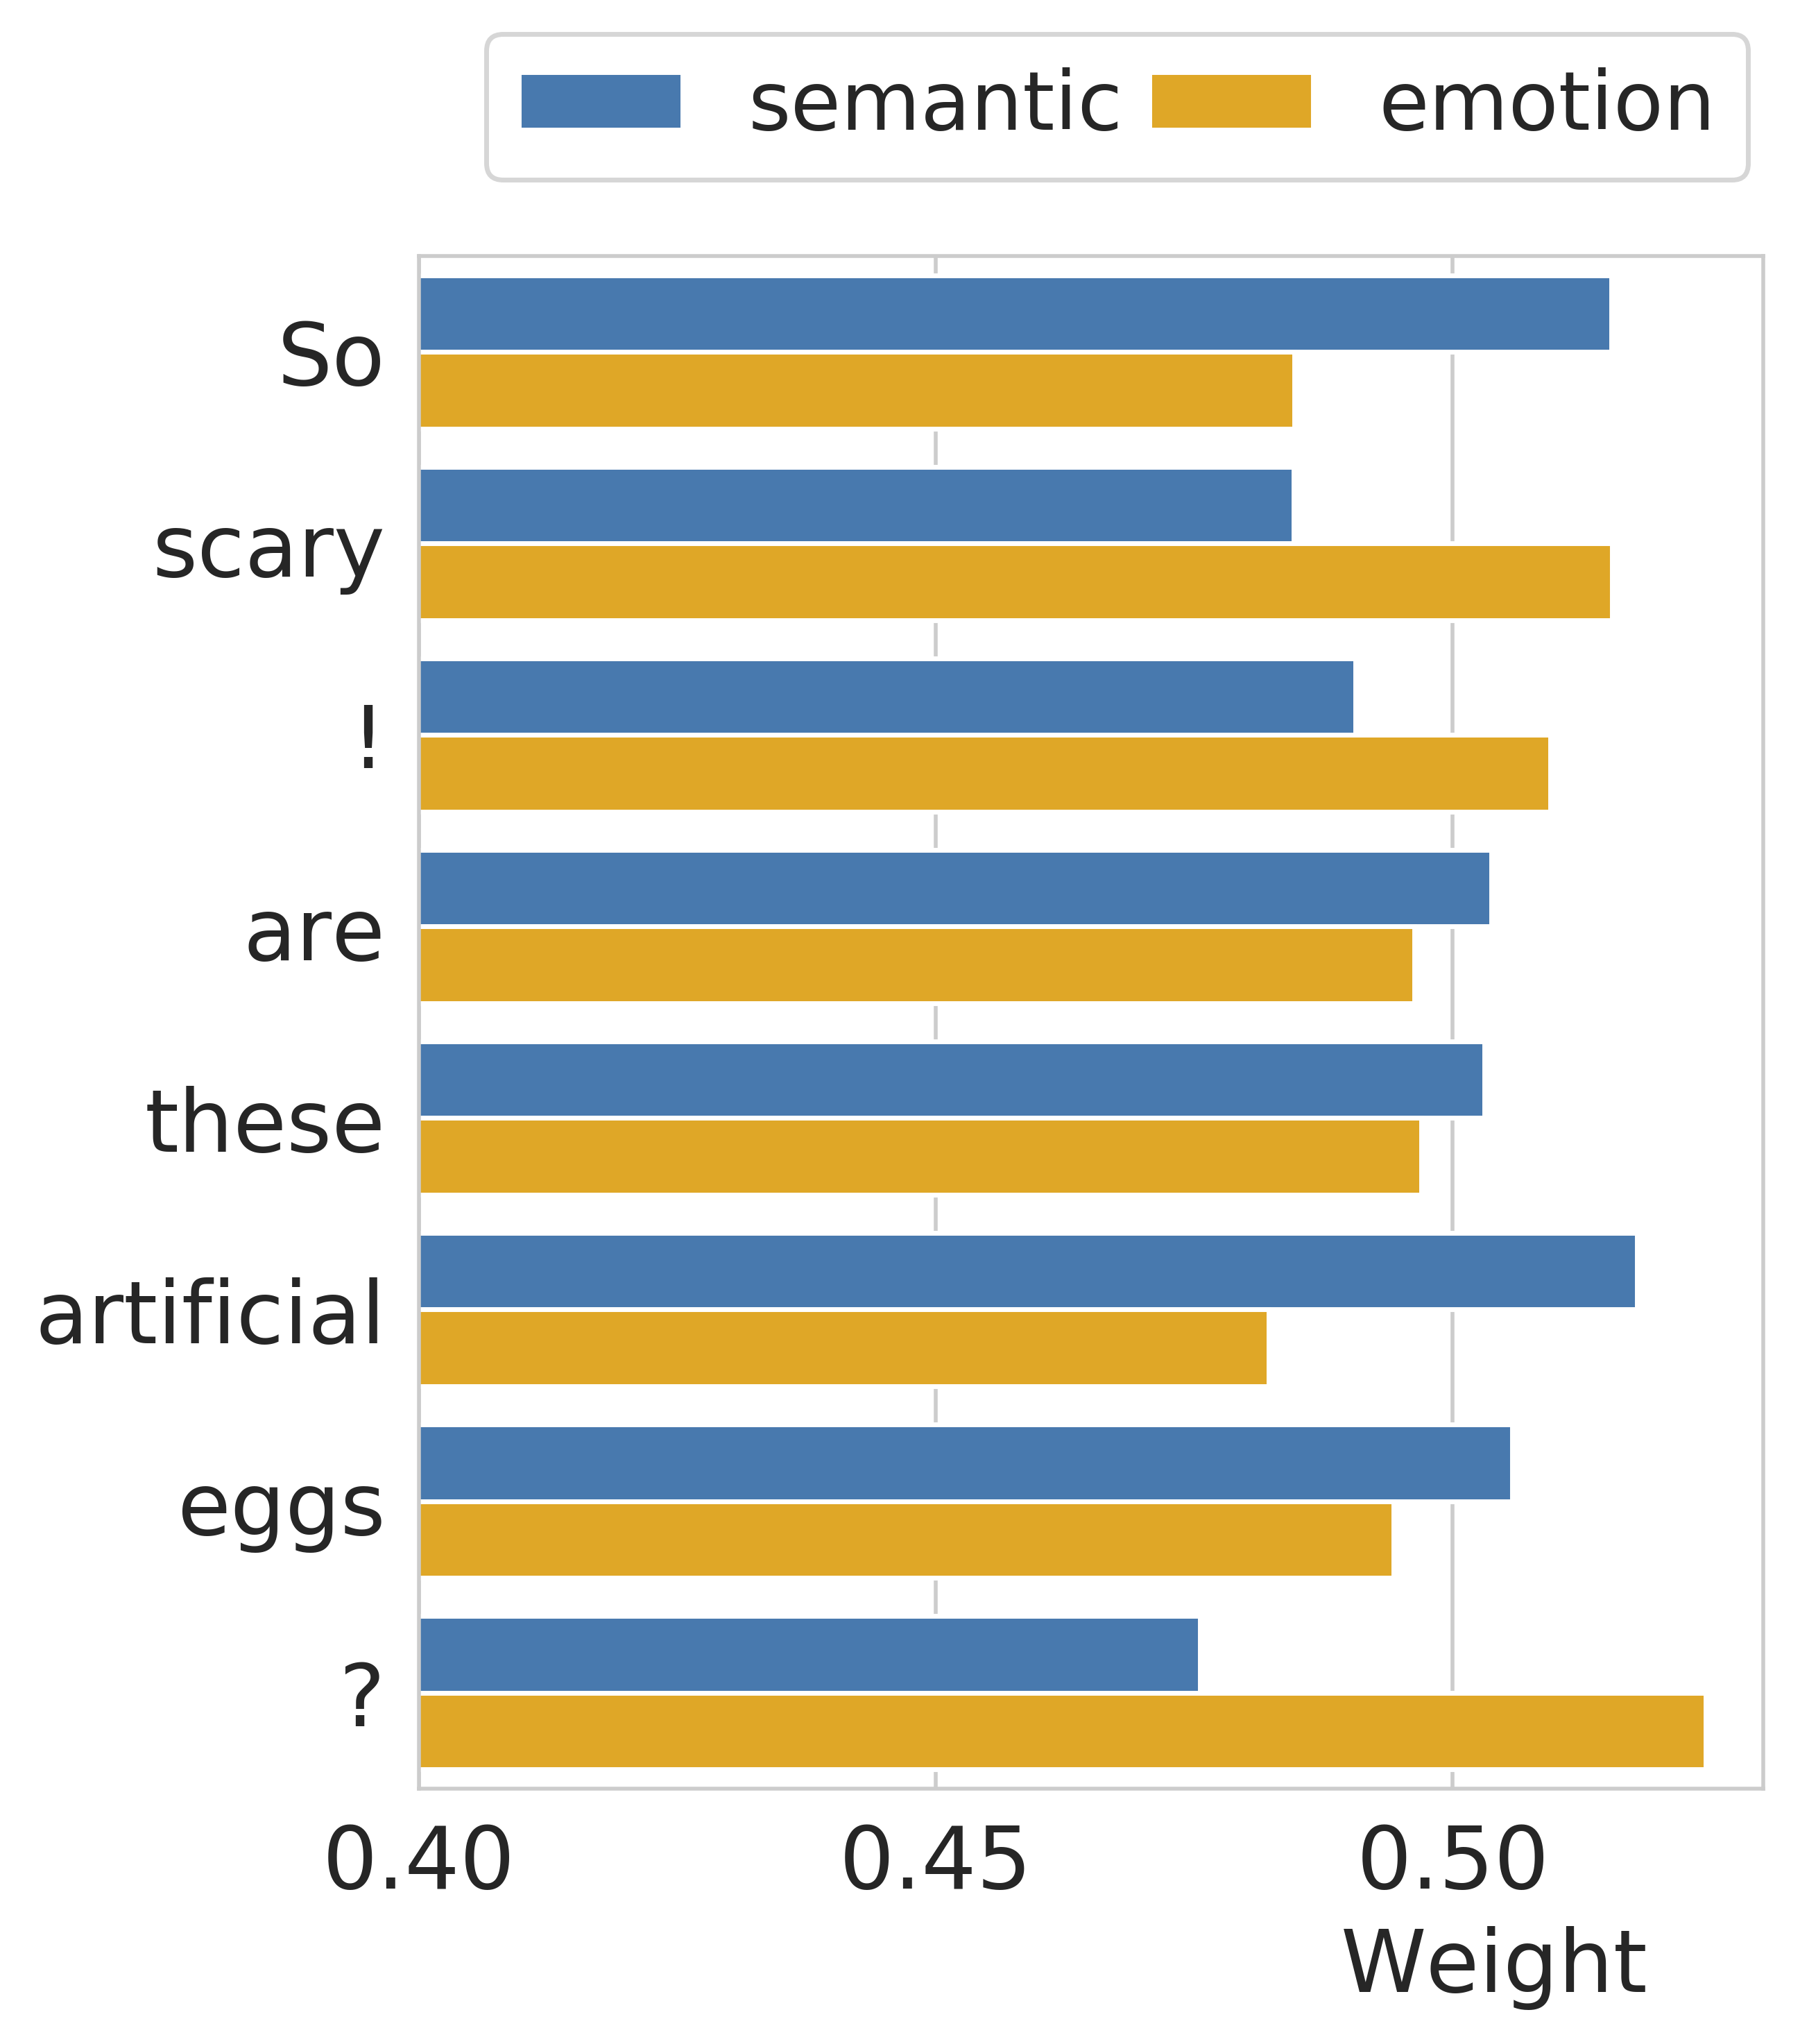
\includegraphics[width=1.5in]{./Figure/case1.png}}
		\end{minipage}
		\begin{minipage}[t]{0.23\textwidth}
			\subfloat[Fake news whose comment module is top Gate\_M weighted.]{\label{Fig:casesduty2}%%
				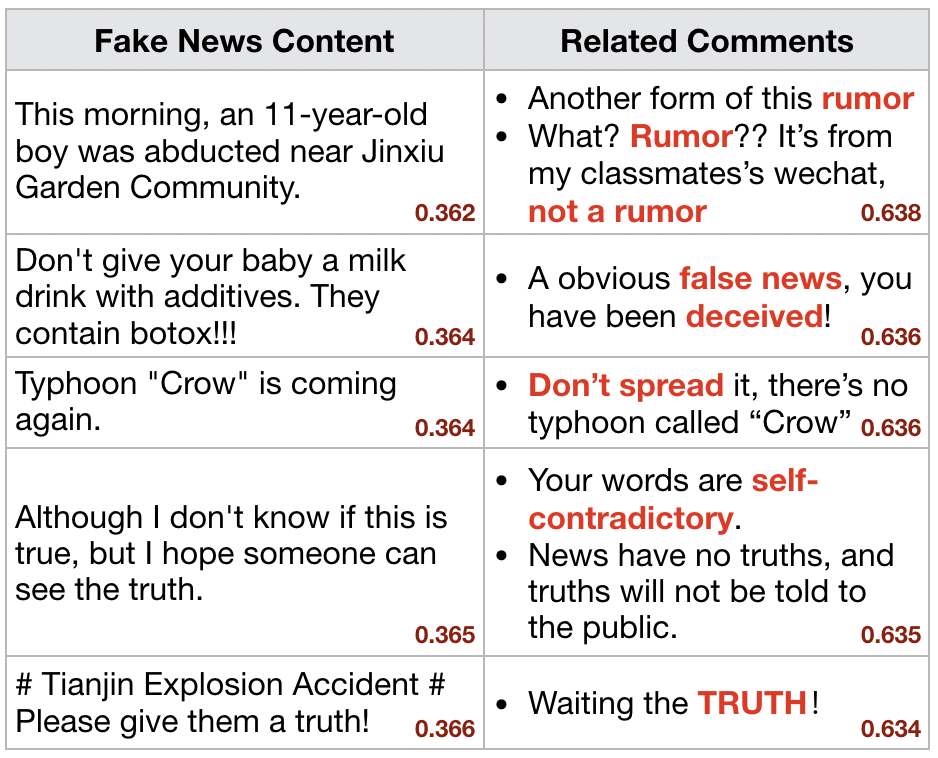
\includegraphics[width=1.8in]{./Figure/case2.png}}
		\end{minipage}
		
		\caption{Analysis of weights in Gate\_C and Gate\_M: (a) Gate\_C Weights of each word in a sentence; and (b) Fake news whose comment modules are top Gate\_M weighted.}
		\label{Fig:casestudy}
		\vspace{-0.35cm}
	\end{figure}
	
	\section{Conclusion}
	In this paper, we propose a end-to-end emotion-based fake news detection framework, {\m}, which incorporate the publisher emotion and the social emotion in fake news detection simultaneously. We use content module and comment module to learn semantic and emotion information from the publisher and users. Technically, we adopt embedding for emotion representation for each word and propose three types of gates for fusion at different levels to fully explore emotion information.  Extensive experiments on microblogs demonstrate that the proposed {\m} model is effective for detecting fake news and outperforms the state-of-art  fake news detection methods.
	
	\appendix
%	\newpage
	%% The file named.bst is a bibliography style file for BibTeX 0.99c
	\bibliographystyle{named}
	\bibliography{ijcai19}
	
\end{document}